\documentclass{beamer}\usepackage[]{graphicx}\usepackage[]{color}
% maxwidth is the original width if it is less than linewidth
% otherwise use linewidth (to make sure the graphics do not exceed the margin)
\makeatletter
\def\maxwidth{ %
  \ifdim\Gin@nat@width>\linewidth
    \linewidth
  \else
    \Gin@nat@width
  \fi
}
\makeatother

\definecolor{fgcolor}{rgb}{0.345, 0.345, 0.345}
\newcommand{\hlnum}[1]{\textcolor[rgb]{0.686,0.059,0.569}{#1}}%
\newcommand{\hlstr}[1]{\textcolor[rgb]{0.192,0.494,0.8}{#1}}%
\newcommand{\hlcom}[1]{\textcolor[rgb]{0.678,0.584,0.686}{\textit{#1}}}%
\newcommand{\hlopt}[1]{\textcolor[rgb]{0,0,0}{#1}}%
\newcommand{\hlstd}[1]{\textcolor[rgb]{0.345,0.345,0.345}{#1}}%
\newcommand{\hlkwa}[1]{\textcolor[rgb]{0.161,0.373,0.58}{\textbf{#1}}}%
\newcommand{\hlkwb}[1]{\textcolor[rgb]{0.69,0.353,0.396}{#1}}%
\newcommand{\hlkwc}[1]{\textcolor[rgb]{0.333,0.667,0.333}{#1}}%
\newcommand{\hlkwd}[1]{\textcolor[rgb]{0.737,0.353,0.396}{\textbf{#1}}}%
\let\hlipl\hlkwb

\usepackage{framed}
\makeatletter
\newenvironment{kframe}{%
 \def\at@end@of@kframe{}%
 \ifinner\ifhmode%
  \def\at@end@of@kframe{\end{minipage}}%
  \begin{minipage}{\columnwidth}%
 \fi\fi%
 \def\FrameCommand##1{\hskip\@totalleftmargin \hskip-\fboxsep
 \colorbox{shadecolor}{##1}\hskip-\fboxsep
     % There is no \\@totalrightmargin, so:
     \hskip-\linewidth \hskip-\@totalleftmargin \hskip\columnwidth}%
 \MakeFramed {\advance\hsize-\width
   \@totalleftmargin\z@ \linewidth\hsize
   \@setminipage}}%
 {\par\unskip\endMakeFramed%
 \at@end@of@kframe}
\makeatother

\definecolor{shadecolor}{rgb}{.97, .97, .97}
\definecolor{messagecolor}{rgb}{0, 0, 0}
\definecolor{warningcolor}{rgb}{1, 0, 1}
\definecolor{errorcolor}{rgb}{1, 0, 0}
\newenvironment{knitrout}{}{} % an empty environment to be redefined in TeX

\usepackage{alltt}

\def\currentCourse{Data anaysis and Unsupervised Learning}
\def\currentInstitute{MAP 573, 2020 -- Julien Chiquet}
\def\currentLogo{../common_figs/logo_X}
\def\currentDate{\'Ecole Polytechnique, Autumn semester, 2020}
\def\currentChapter{Dimensionality Reduction: Beyond PCA and Non Linear Methods}


% THEME BEAMER
\usepackage{../beamer_theme}

\graphicspath{{figures/},{../common_figs/}}

\usepackage{multirow}
\usepackage{tikz}
\usepackage[vlined]{algorithm2e}

\pgfdeclareimage[width=.5cm]{computer}{computer.png}

% \usetikzlibrary{calc,shapes,backgrounds,arrows,automata,shadows,positioning}
% \tikzstyle{every state}=[fill=red,draw=none,scale=0.7,font=\small,text=white]
% \tikzstyle{every edge}=[-,shorten >=1pt,auto,thin,draw]
% \tikzstyle{alertstate}=[fill=bleu]
% \definecolor{genecolor}{RGB}{94,135,173}

\title{\currentCourse}

\subtitle{\huge\currentChapter\normalsize}

\institute{\currentInstitute}

\date{\currentDate}



\AtBeginSection{
  \begin{frame}<beamer>
    \frametitle{Outline}
    \framesubtitle{\insertpart}
    \tableofcontents[currentsection,currentsubsection, subsectionstyle=show/shaded/hide]  
  \end{frame}
}

\AtBeginSubsection{
  \begin{frame}<beamer>
    \frametitle{Outline}
    \framesubtitle{\insertpart}
    \tableofcontents[currentsection,currentsubsection, subsectionstyle=show/shaded/hide]  
  \end{frame}
}

\AtBeginSubsubsection{
  \begin{frame}<beamer>
    \frametitle{Outline}
    \framesubtitle{\insertpart}
    \tableofcontents[currentsection,currentsubsection, subsectionstyle=show/shaded/hide]  
  \end{frame}
}

\newcommand{\dotitlepage}{%
  \begin{frame}
    \titlepage
    \vfill
    \begin{center}
        \scriptsize\url{https://jchiquet.github.io/MAP573}
    \end{center}
    \vfill
    \includegraphics[width=2cm]{\currentLogo}\hfill
    \includegraphics[width=2.5cm]{logo_inra}
  \end{frame}
  %
}

\newcommand{\dotoc}{%
  \begin{frame}
    \frametitle{Outline}
    \tableofcontents[currentsection,
    sectionstyle=show/show,
    subsectionstyle=hide]
  \end{frame}
  %
}

\graphicspath{{figs/}}
\IfFileExists{upquote.sty}{\usepackage{upquote}}{}
\begin{document}

\dotitlepage

%% ====================================================================
\part{Introduction}
%% ====================================================================

\begin{frame}[fragile]
  \partpage

\paragraph{Packages required for reproducing the slides}
\begin{knitrout}\scriptsize
\definecolor{shadecolor}{rgb}{0.969, 0.969, 0.969}\color{fgcolor}\begin{kframe}
\begin{alltt}
\hlkwd{library}\hlstd{(tidyverse)}  \hlcom{# opinionated collection of packages for data manipulation}
\hlkwd{library}\hlstd{(GGally)}     \hlcom{# extension to ggplot vizualization system}
\hlkwd{library}\hlstd{(FactoMineR)} \hlcom{# PCA and oter linear method for dimension reduction}
\hlkwd{library}\hlstd{(factoextra)} \hlcom{# fancy plotting for FactoMineR output }
\hlkwd{library}\hlstd{(NMF)}        \hlcom{# Non-Negative Matrix factorisation}
\hlkwd{library}\hlstd{(kernlab)}    \hlcom{# Kernel PCA}
\hlkwd{library}\hlstd{(MASS)}       \hlcom{# Various statistical too, including MDS}
\hlkwd{library}\hlstd{(Rtsne)}      \hlcom{# tSNE implementation in R }
\hlkwd{library}\hlstd{(umap)}       \hlcom{# Uniform Manifold Approximation and Projection}
\hlkwd{theme_set}\hlstd{(}\hlkwd{theme_bw}\hlstd{())}
\end{alltt}
\end{kframe}
\end{knitrout}

\end{frame}

\begin{frame}[fragile]
  \frametitle{Companion data set: 'scRNA'}
  \framesubtitle{Subsamples of normalized Single-Cell RNAseq}

\begin{block}{Description: \textcolor{black}{\it subsample of a large data set}}
\small Gene-level expression of 100 representative genes for a collection of 301 cells 
spreaded in 11 cell-lines. Original transcription data are measured by counts obtained by 
\textit{RNAseq} and normalized to be close to a Gaussian distribution.\\

\begin{scriptsize}
\begin{thebibliography}{9}
\bibitem{pollen} Pollen, Alex A., et al. \textcolor{black}{Low-coverage single-cell mRNA sequencing reveals cellular heterogeneity and activated signaling pathways in developing cerebral cortex.} \newblock Nature biotechnology 32.10 (2014): 1053.
\end{thebibliography}
\end{scriptsize}
\end{block}

\begin{figure}
  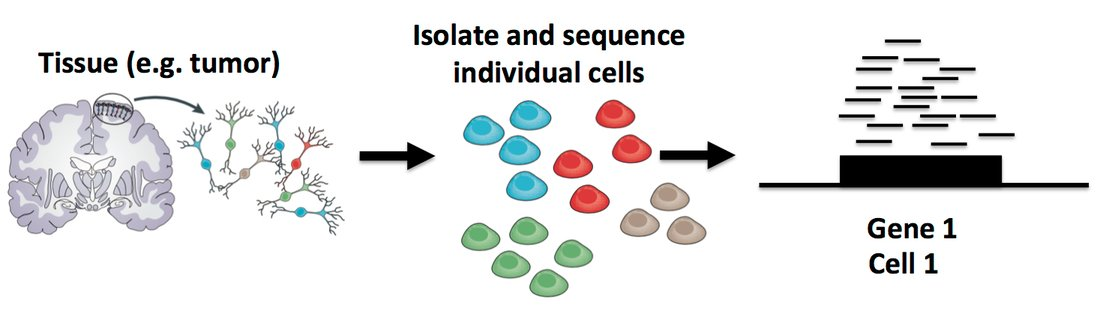
\includegraphics[width=.9\textwidth]{figures/scRNA-overview}
  \caption{Single Cell RNA sequnencing data: general principle -- {\tiny source: Stephanie Hicks}}
\end{figure}

\end{frame}

\begin{frame}[fragile]
  \frametitle{Companion data set: 'scRNA'}
  \framesubtitle{Brief data summary I}

\paragraph{Data manipulation}

\begin{knitrout}\scriptsize
\definecolor{shadecolor}{rgb}{0.969, 0.969, 0.969}\color{fgcolor}\begin{kframe}
\begin{alltt}
\hlkwd{load}\hlstd{(}\hlstr{"../../data/scRNA.RData"}\hlstd{)}
\hlstd{scRNA} \hlkwb{<-}  \hlstd{pollen}\hlopt{$}\hlstd{data} \hlopt \hlkwd{t}\hlstd{()} \hlopt \hlkwd{as_tibble}\hlstd{()} \hlopt
  \hlkwd{add_column}\hlstd{(}\hlkwc{cell_type} \hlstd{= pollen}\hlopt{$}\hlstd{celltypes)}
\end{alltt}
\end{kframe}
\end{knitrout}

\paragraph{Cell types}

\begin{knitrout}\scriptsize
\definecolor{shadecolor}{rgb}{0.969, 0.969, 0.969}\color{fgcolor}\begin{kframe}
\begin{alltt}
\hlstd{scRNA} \hlopt \hlstd{dplyr}\hlopt{::}\hlkwd{select}\hlstd{(cell_type)} \hlopt \hlkwd{summary}\hlstd{()}  \hlopt \hlstd{knitr}\hlopt{::}\hlkwd{kable}\hlstd{()}
\end{alltt}
\end{kframe}
\begin{tabular}{l|l}
\hline
  &   cell\_type\\
\hline
 & HL60   :54\\
\hline
 & K562   :42\\
\hline
 & Kera   :40\\
\hline
 & BJ     :37\\
\hline
 & GW16   :26\\
\hline
 & hiPSC  :24\\
\hline
 & (Other):78\\
\hline
\end{tabular}


\end{knitrout}

\end{frame}

\begin{frame}[fragile]
  \frametitle{Companion data set II: 'scRNA'}
  \framesubtitle{Brief data summary II}

\paragraph{Histogram of normalized expression}

\begin{knitrout}\scriptsize
\definecolor{shadecolor}{rgb}{0.969, 0.969, 0.969}\color{fgcolor}\begin{kframe}
\begin{alltt}
\hlstd{scRNA} \hlopt \hlstd{dplyr}\hlopt{::}\hlkwd{select}\hlstd{(}\hlopt{-}\hlstd{cell_type)} \hlopt \hlkwd{pivot_longer}\hlstd{(}\hlkwd{everything}\hlstd{())} \hlopt
  \hlkwd{ggplot}\hlstd{()} \hlopt{+} \hlkwd{aes}\hlstd{(}\hlkwc{x} \hlstd{= value,} \hlkwc{fill} \hlstd{= name)} \hlopt{+} \hlkwd{geom_histogram}\hlstd{(}\hlkwc{show.legend} \hlstd{=} \hlnum{FALSE}\hlstd{)}
\end{alltt}
\end{kframe}
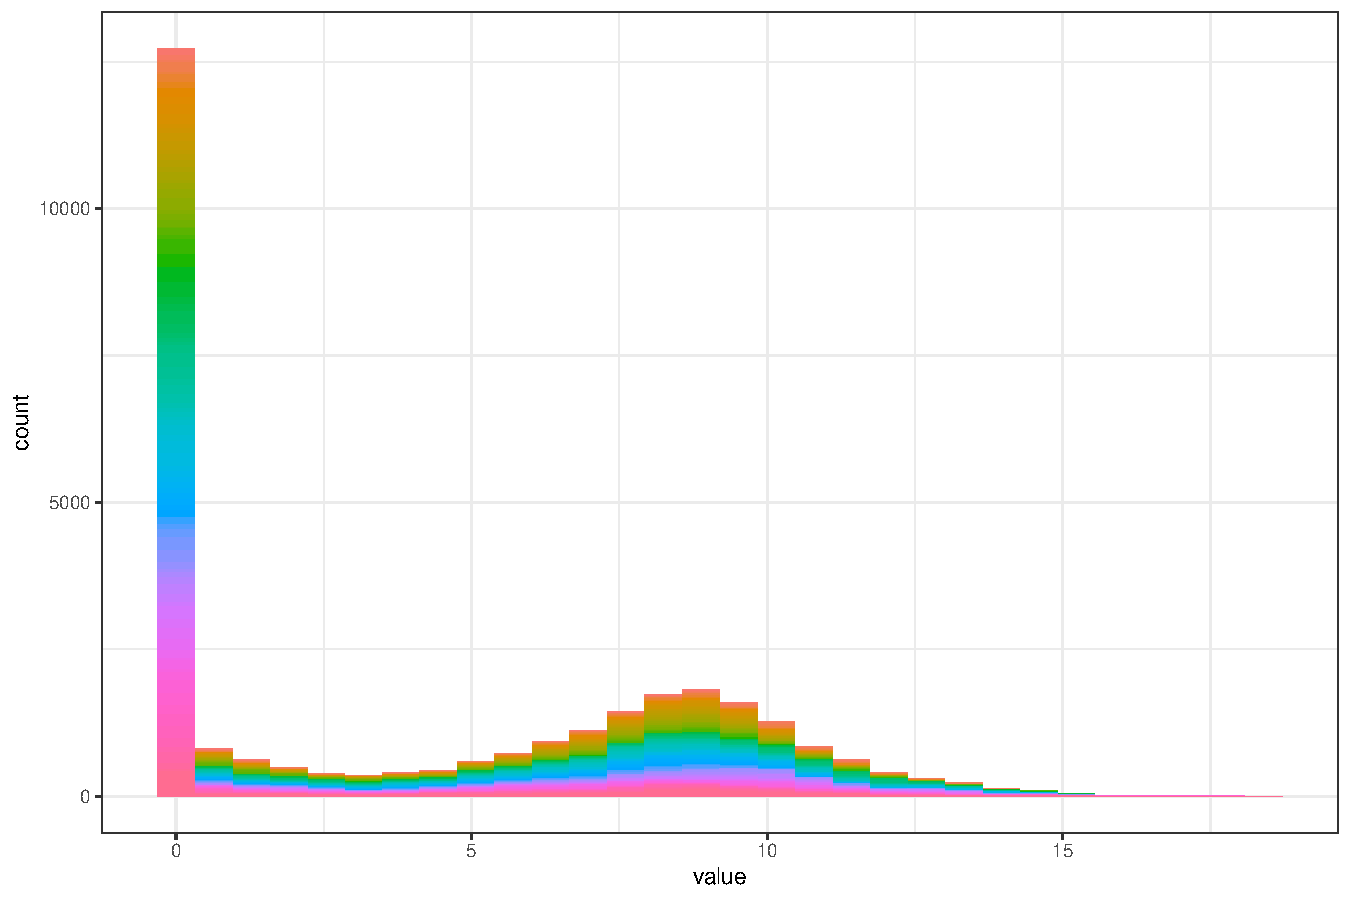
\includegraphics[width=.8\textwidth]{figures/scRNA_expressions-1} 

\end{knitrout}
\end{frame}

\begin{frame}[fragile]
  \frametitle{Companion data set: 'scRNA'}
  \framesubtitle{PCA}

\begin{knitrout}\scriptsize
\definecolor{shadecolor}{rgb}{0.969, 0.969, 0.969}\color{fgcolor}\begin{kframe}
\begin{alltt}
\hlstd{scRNA} \hlopt \hlstd{FactoMineR}\hlopt{::}\hlkwd{PCA}\hlstd{(}\hlkwc{graph} \hlstd{=} \hlnum{FALSE}\hlstd{,} \hlkwc{quali.sup} \hlstd{=} \hlkwd{which}\hlstd{(}\hlkwd{colnames}\hlstd{(scRNA)} \hlopt{==} \hlstr{"cell_type"}\hlstd{))} \hlopt
  \hlstd{factoextra}\hlopt{::}\hlkwd{fviz_pca_biplot}\hlstd{(}\hlkwc{select.var} \hlstd{=} \hlkwd{list}\hlstd{(}\hlkwc{contrib} \hlstd{=} \hlnum{30}\hlstd{),} \hlkwc{habillage} \hlstd{=} \hlstr{"cell_type"}\hlstd{)}
\end{alltt}
\end{kframe}
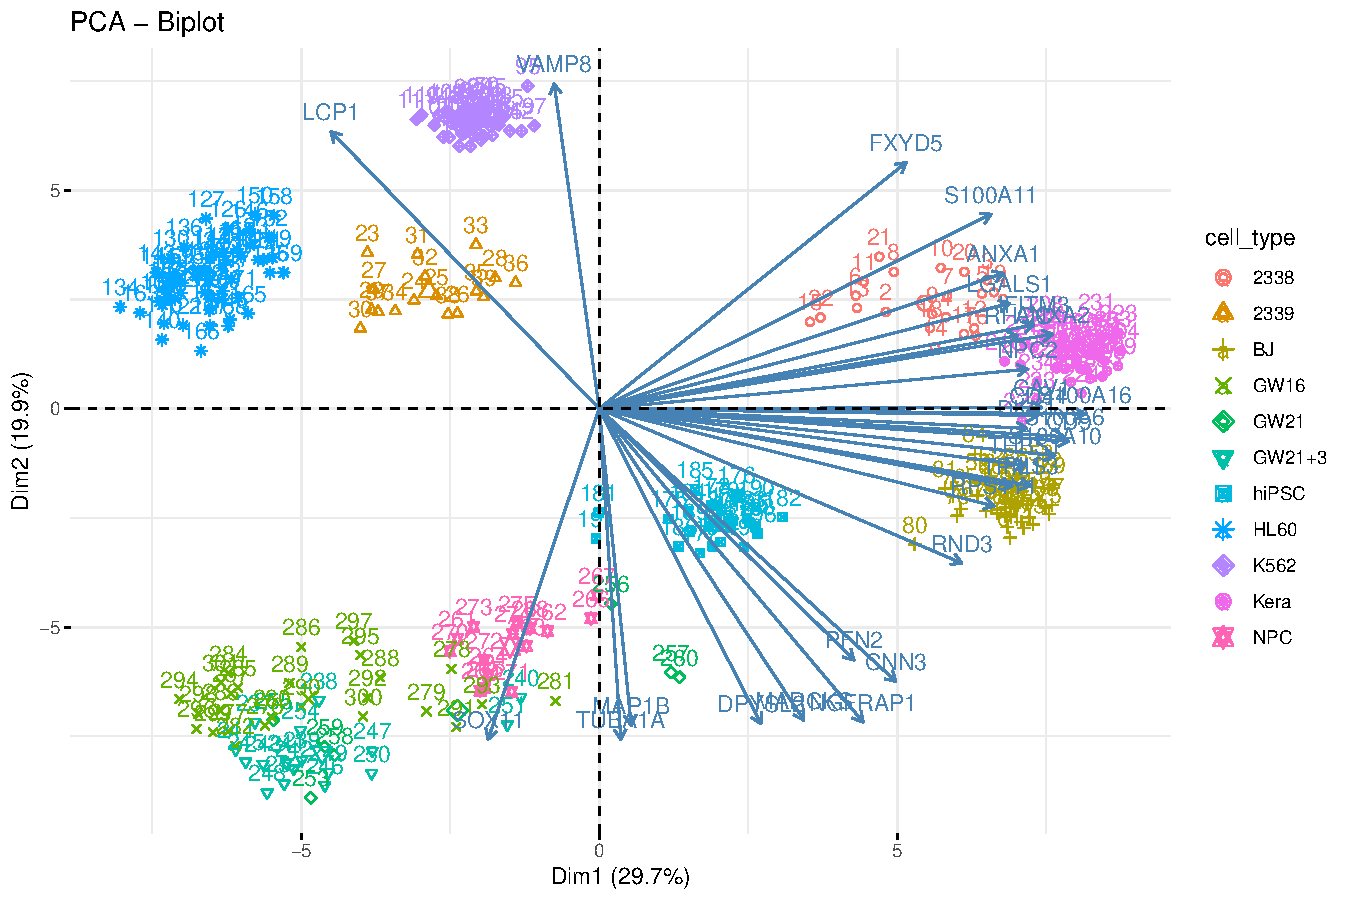
\includegraphics[width=.8\textwidth]{figures/scRNA_PCA-1} 

\end{knitrout}

\end{frame}

\begin{frame}
  \frametitle{PCA (and linear methods) limitations}

  \begin{block}{Account for complex pattern}
    \begin{itemize}
      \item Linear methods are powerful for \alert{\bf planar structures}
      \item May fail at describing \alert{\bf manifolds}
    \end{itemize}
  \end{block}
  
  \begin{block}{Preserve local geometry}
    \begin{itemize}
      \item High dimensional data are characterized by \alert{\bf multiscale properties} (local / global structures)
      \item Non Linear projection helps at preserving \alert{\bf local characteristics} of distances
    \end{itemize}
  \end{block}

  \vfill
  
   \begin{figure}
     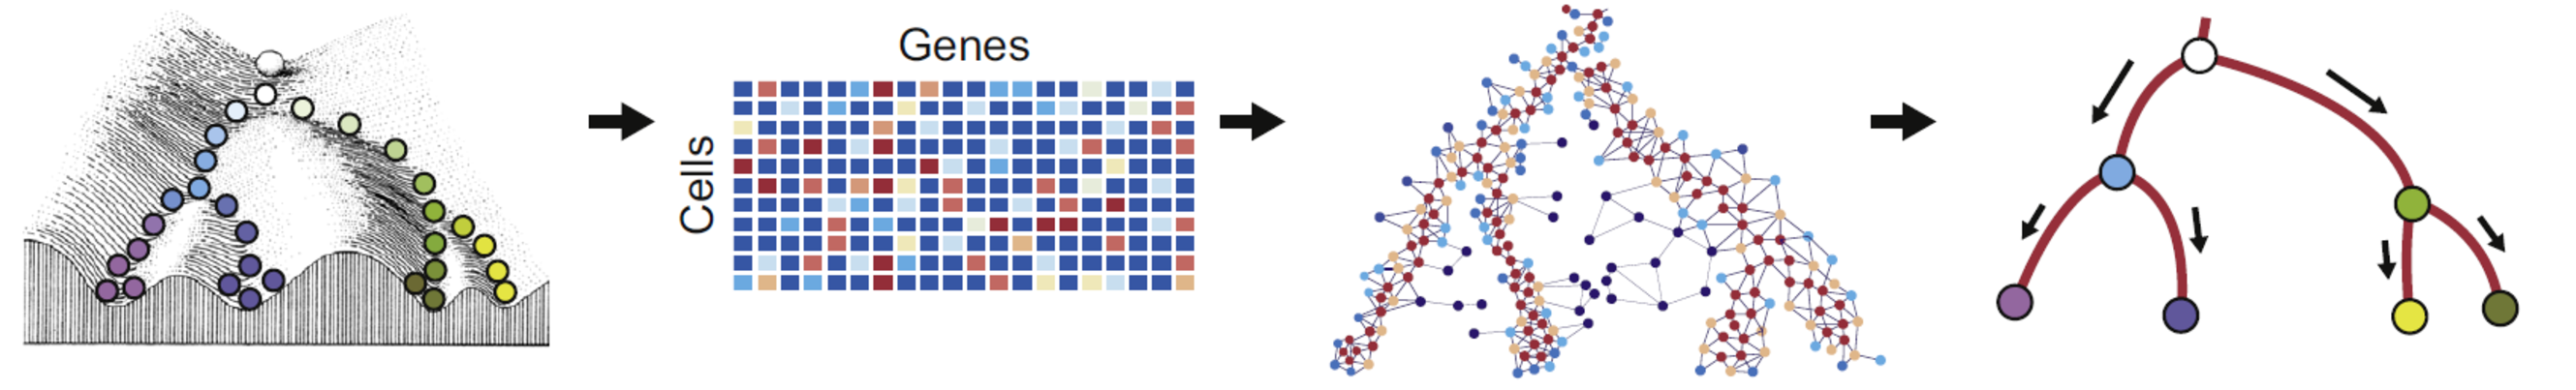
\includegraphics[scale=0.25]{figures/manifold.pdf}
     \caption{\small Intuition of manifolds and geometry underlying sc-data -- {\tiny source: F. Picard}}
   \end{figure}

\end{frame}

\begin{frame}[fragile]
  \frametitle{Companion data set II: 'mollusk'}
  \framesubtitle{Abundance table (Species counts spread in various sites)}

\begin{block}{Description: \textcolor{black}{\it small size count data}}
\small Abundance of 32 mollusk species in 163 samples. For each sample, 4 additional covariates are known. \\

\begin{scriptsize}
\begin{thebibliography}{9}
\bibitem{mollusk} Richardot-Coulet, M., Chessel D. and Bournaud M. \textcolor{black}{Typological value of the benthos of old beds of a large river. Methodological approach. Archiv fùr Hydrobiologie, 107.}
\end{thebibliography}
\end{scriptsize}
\end{block}

\begin{knitrout}\scriptsize
\definecolor{shadecolor}{rgb}{0.969, 0.969, 0.969}\color{fgcolor}\begin{kframe}
\begin{alltt}
\hlkwd{library}\hlstd{(PLNmodels);} \hlkwd{data}\hlstd{(mollusk)}
\hlstd{mollusk} \hlkwb{<-}
  \hlkwd{prepare_data}\hlstd{(mollusk}\hlopt{$}\hlstd{Abundance, mollusk}\hlopt{$}\hlstd{Covariate[}\hlkwd{c}\hlstd{(}\hlstr{"season"}\hlstd{,} \hlstr{"site"}\hlstd{)])} \hlopt
  \hlstd{dplyr}\hlopt{::}\hlkwd{select}\hlstd{(}\hlopt{-}\hlstd{Offset)} \hlopt
  \hlkwd{as_tibble}\hlstd{()} \hlopt
  \hlkwd{distinct}\hlstd{()} \hlcom{# remove duplicates}
\hlstd{mollusk} \hlkwb{<-} \hlkwd{cbind}\hlstd{(mollusk}\hlopt{$}\hlstd{Abundance, mollusk[}\hlkwd{c}\hlstd{(}\hlstr{"season"}\hlstd{,} \hlstr{"site"}\hlstd{)])}
\end{alltt}
\end{kframe}
\end{knitrout}

\paragraph{External Covariates}

\begin{knitrout}\scriptsize
\definecolor{shadecolor}{rgb}{0.969, 0.969, 0.969}\color{fgcolor}\begin{kframe}
\begin{alltt}
\hlstd{mollusk} \hlopt \hlstd{dplyr}\hlopt{::}\hlkwd{select}\hlstd{(site, season)} \hlopt \hlkwd{summary}\hlstd{()} \hlopt \hlkwd{t}\hlstd{()} \hlopt \hlstd{knitr}\hlopt{::}\hlkwd{kable}\hlstd{()}
\end{alltt}
\end{kframe}
\begin{tabular}{l|l|l|l|l|l|l|l}
\hline
  &  &  &  &  &  &  & \\
\hline
site & Negria1  :24 & Negria2  :24 & Pecheurs1:24 & Pecheurs2:23 & GGravier1:21 & GGravier3:18 & (Other)  :24\\
\hline
season & automn:41 & spring:43 & summer:44 & winter:30 & NA & NA & NA\\
\hline
\end{tabular}


\end{knitrout}

\end{frame}

\begin{frame}[fragile]
  \frametitle{Companion data set: 'mollusk'}
  \framesubtitle{Brief data summary II}

\paragraph{Histogram of raw counts}

\begin{knitrout}\scriptsize
\definecolor{shadecolor}{rgb}{0.969, 0.969, 0.969}\color{fgcolor}\begin{kframe}
\begin{alltt}
\hlstd{mollusk} \hlopt \hlstd{dplyr}\hlopt{::}\hlkwd{select}\hlstd{(}\hlopt{-}\hlstd{site,} \hlopt{-}\hlstd{season)} \hlopt
  \hlkwd{pivot_longer}\hlstd{(}\hlkwd{everything}\hlstd{())} \hlopt
  \hlkwd{ggplot}\hlstd{()} \hlopt{+} \hlkwd{aes}\hlstd{(}\hlkwc{x} \hlstd{= value,} \hlkwc{fill} \hlstd{= name)} \hlopt{+} \hlkwd{geom_histogram}\hlstd{(}\hlkwc{show.legend} \hlstd{=} \hlnum{FALSE}\hlstd{)}
\end{alltt}
\end{kframe}

\includegraphics[width=.8\textwidth]{figures/mollusc_abundance-1} 

\end{knitrout}
\end{frame}

\begin{frame}[fragile]
  \frametitle{Companion data set: 'mollusk'}
  \framesubtitle{PCA}

\begin{knitrout}\scriptsize
\definecolor{shadecolor}{rgb}{0.969, 0.969, 0.969}\color{fgcolor}\begin{kframe}
\begin{alltt}
\hlstd{mollusk} \hlopt \hlkwd{PCA}\hlstd{(}\hlkwc{graph} \hlstd{=} \hlnum{FALSE}\hlstd{,} \hlkwc{quali.sup} \hlstd{=} \hlkwd{which}\hlstd{(}\hlkwd{map_lgl}\hlstd{(mollusk, is.factor)))} \hlopt
  \hlkwd{fviz_pca_biplot}\hlstd{(}\hlkwc{select.var} \hlstd{=} \hlkwd{list}\hlstd{(}\hlkwc{contrib} \hlstd{=} \hlnum{5}\hlstd{),} \hlkwc{habillage} \hlstd{=} \hlstr{"site"}\hlstd{)}
\end{alltt}
\end{kframe}
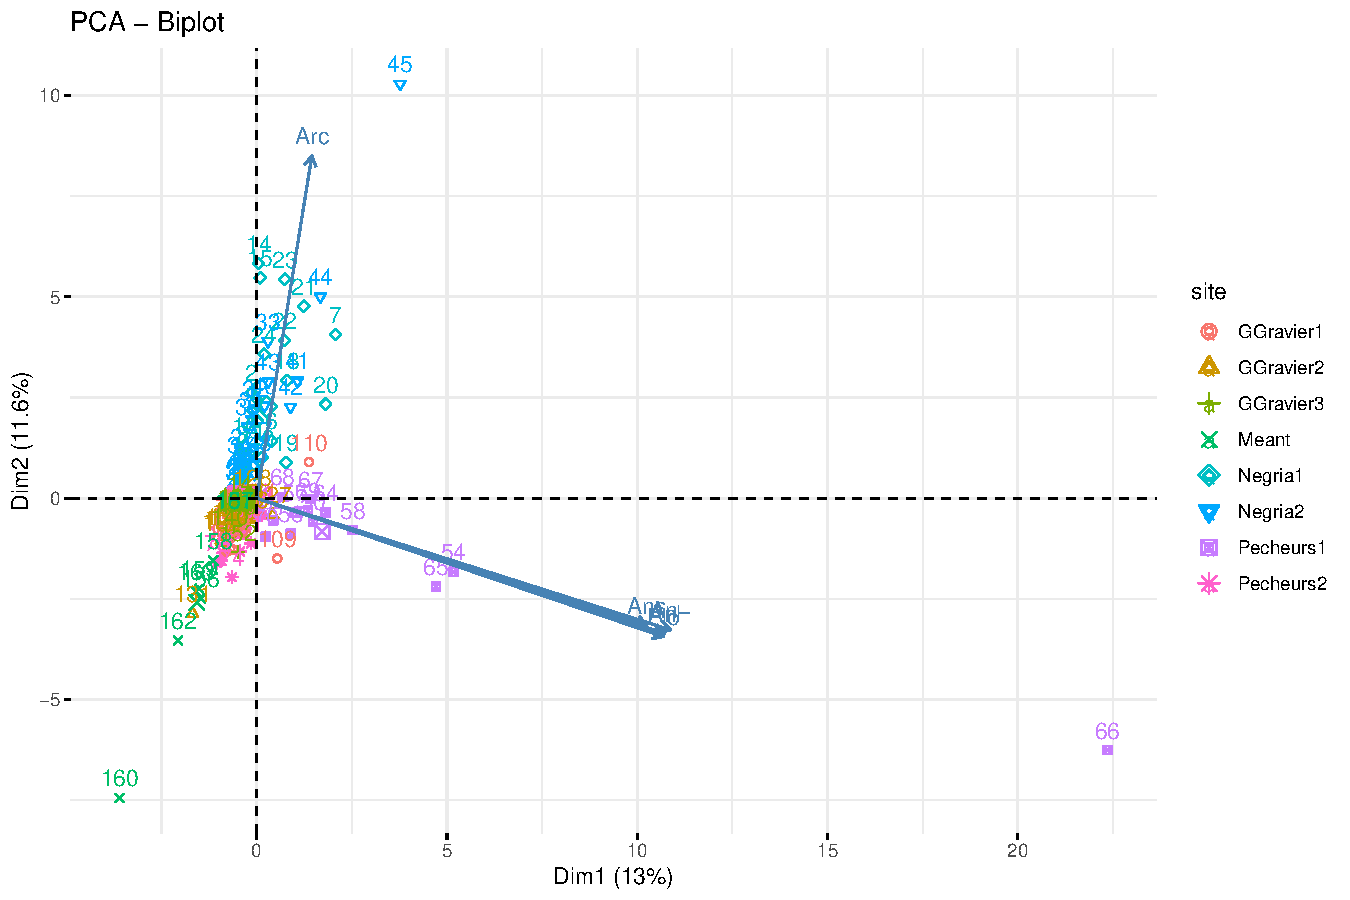
\includegraphics[width=.8\textwidth]{figures/mollusk_PCA-1} 

\end{knitrout}

\end{frame}

\begin{frame}
  \frametitle{PCA (and linear methods) limitations}

  \begin{block}{Account for complex data distribution}
    \begin{itemize}
      \item Linear methods /PCA are tied to an hidden \alert{\bf Gaussian assumption}
      \item Fail with \alert{\bf Count data}
      \item Fail with \alert{\bf Skew data}
    \end{itemize}
  \end{block}
  
  \vfill
  
  \begin{block}{Possible solutions}
    \begin{itemize}
      \item Probabilistic (non Gaussian) models
      \item Need transformed (non-linear) input space
    \end{itemize}
  \end{block}
  
  \end{frame}

\begin{frame}
  \frametitle{Dimension reduction: revisiting the problem setup}

    \begin{block}{Settings}
      \begin{itemize}
        \item \alert{Training data} : $\mathcal{D}=\{\bx_1,\ldots,\bx_n\} \in \Rset^p$,   (i.i.d.)
        \item Space $\Rset^p$ of possibly high dimension $(n \ll p)$
      \end{itemize}
    \end{block}

    \vfill
    
    \begin{block}{Dimension Reduction Map}
       Construct a map $\Phi$ from the space $\Rset^{p}$ into a space $\Rset^{q}$ of \alert{smaller dimension}:
      \begin{align*}
          \Phi:\quad & \Rset^p \to \Rset^{q}, q \ll p\\
                     & \bx \mapsto \Phi(\bx)
      \end{align*}
    \end{block}
    
\end{frame}

\begin{frame}
  \frametitle{How should we design/construct $\Phi$?}

  \paragraph{Criterion}
  \begin{itemize}
    \item Geometrical approach (\alert{\bf see slides on PCA})
    \item Reconstruction error
    \item Relationship preservation
  \end{itemize}

  \vfill
  
  \paragraph{Form of the map $\Phi$}
  \begin{itemize}
    \item \alert{\bf Linear} or \alert{\bf non-linear ?}
    \item tradeoff between  interpretability and \alert{\bf versatility ?}
    \item tradeoff between  \alert{\bf high} or low computational resource
  \end{itemize}

\end{frame}




%% ====================================================================
\part{Non-linear methods}
%% ====================================================================
\begin{frame}
  \partpage
\end{frame}

\section{Motivated by reconstruction error}

\subsection{PCA as a matrix factorization}

\begin{frame}
  \frametitle{Reconstruction error approach}

  \begin{enumerate}
    \item  Construct a map $\Phi$ from the space $\Rset^{p}$ into a space $\Rset^{q}$ of \alert{smaller dimension}:
      \begin{align*}
      \Phi:\quad & \Rset^{p} \to \Rset^{q}, q \ll p\\
               & \bx \mapsto \Phi(\bx)
      \end{align*}
    \item Construct $\widetilde{\Phi}$ from $\Rset^{q}$ to $\Rset^{p}$ (\alert{reconstruction formula})
     \item Control an error $\epsilon$ between $\bx$ and its reconstruction $\hat \bx = \tilde{\Phi}(\Phi(\bx))$
  \end{enumerate}

\bigskip

\onslide<2>{
    For instance,  the error measured with th Frobenius between the original data matrix $\bX$ and its approximation:
      \begin{equation*}
        \epsilon(\bX, \hat \bX ) = \left\| \bX - \hat \bX \right\|_F^2  = \sum_{i=1}^n \left\| \bx_i - \tilde{\Phi}(\Phi(\bx_i)) \right\|^2 
      \end{equation*}
}      
\end{frame}

\begin{frame}
\frametitle{Reinterpretation of PCA}

  \begin{block}{PCA model}
       Let $\bV$ be a $p\times q$ matrix whose columns are of $q$ orthonormal vectors.
      \begin{align*}
        \Phi(\bx) & = \bV^\top(\bx-\bmu)  = \tilde\bx \\  
        \bx \simeq \tilde{\Phi}(\tilde\bx) & = \bmu + \bV \tilde\bx
      \end{align*}
      \rsa Model with \alert{\bf Linear assumption + ortho-normality constraints}
    \end{block}

  \begin{block}{PCA reconstruction error}<2>
    \vspace{-.25cm}
    \begin{equation*}
      \minimize_{\bmu \in\Rset^p, \bV\in\mathcal{O}_{p,q}} \sum_{i=1}^n \left\| (\bx_i  - \bmu) + \bV^\top\bV ( \bx_i -\bmu)   \right\|^2
    \end{equation*}
  
  \alert{Solution (explicit)} 
  \begin{itemize}
  \item $\bmu = \bar{\bx}$ the empirical mean
  \item $\bV$  an orthonormal basis of the space spanned by the $q$ first eigenvectors of the empirical covariance matrix
  \end{itemize}
  
  \end{block}
\end{frame}

\begin{frame}
  \frametitle{Important digression: SVD}

  \begin{block}{Singular Value Decomposition (SVD)}
    The SVD of $\mathbf{M}$ a $n\times p$ matrix is the factorization given by
    
    \[ \mathbf{M} =\mathbf{U}\mathbf{D}\mathbf{V}^\top,\]
    where $r = \min(n,p)$ and
    \begin{itemize}
      \item \(\mathbf{D}_{r \times r} = \text{diag}(\delta_1, ...\delta_r)\) is the diagonal matrix of singular values.
      \item \(\mathbf{U}\) is orthonormal, whose columns are eigen vectors of (\(\mathbf{M}\mathbf{M}^T\))
      \item \(\mathbf{V}\) is orthonormal whose columns are eigen vectors of (\(\mathbf{M}^T\mathbf{M}\))
    \end{itemize}
    {\small \rsa Time complexity in $\mathcal{O}(n p q r)$ (less when $k\ll r$ components are required)}
  \end{block}

  \vfill
  
  \begin{block}{Connection with eigen decomposition of the covariance matrix}<2>
    \vspace{-.5cm}
    \begin{align*}
      \mathbf{M}^\top\mathbf{M} & = \mathbf{V} \mathbf{D} \mathbf{U}^\top  \mathbf{U} \mathbf{D} \mathbf{V}^\top \\
        & = \mathbf{V} \mathbf{D}^2 \mathbf{V}^\top  = \mathbf{V} \boldsymbol{\Lambda} \mathbf{V}^\top\\
    \end{align*}
  \end{block}

\end{frame}

%%%%%%%%%%%%%%%%%%%%%%%%%%
%%%%%%%%%%%%%%%%%%%%%%%%%%%%
\begin{frame}{PCA solution is given by SVD of the centered data matrix}

\begin{figure}[ht]
  \centering
  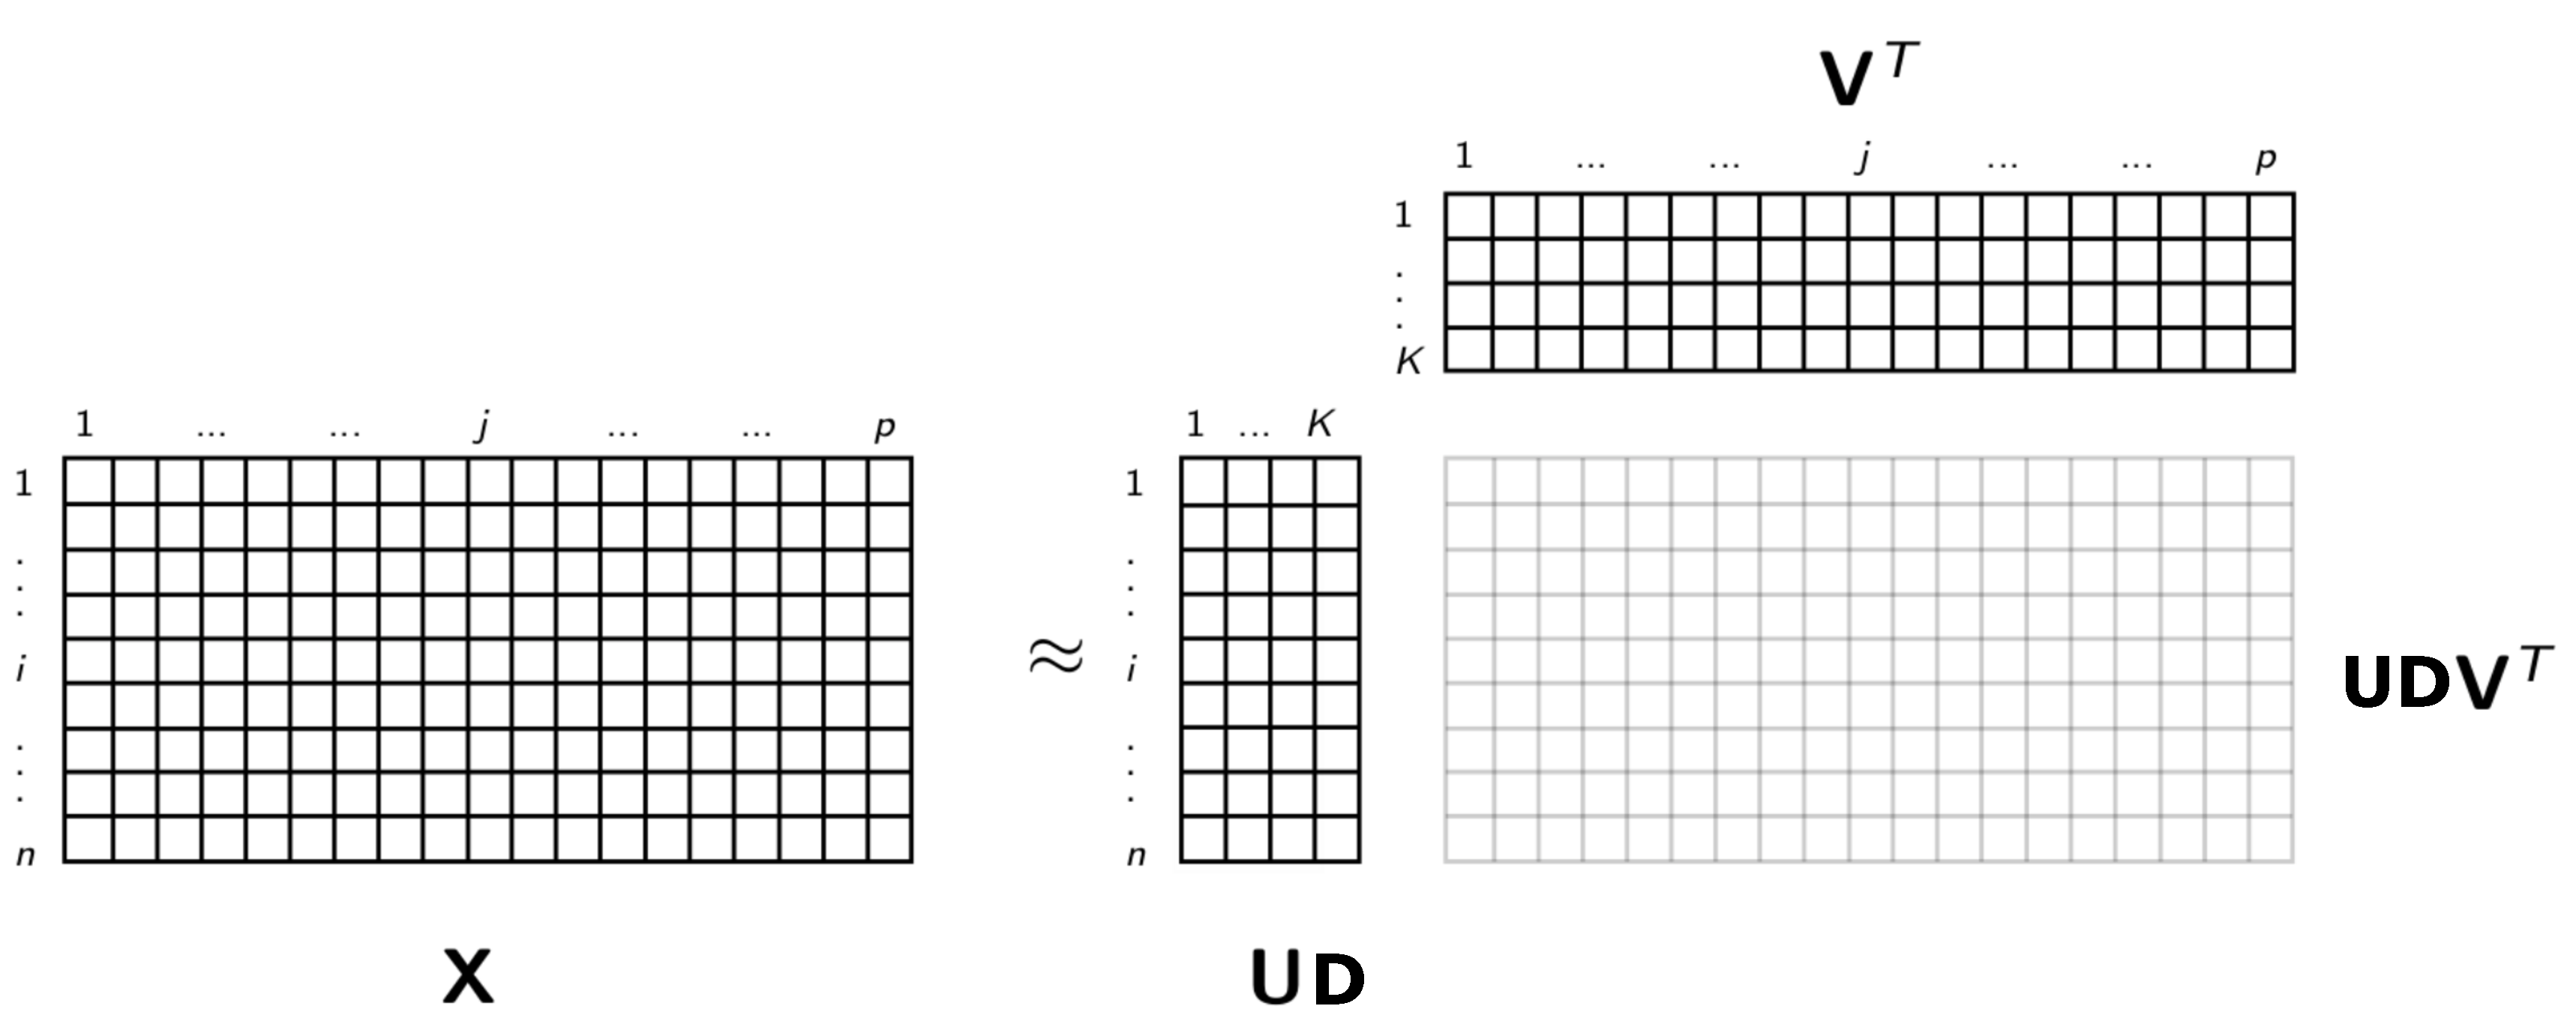
\includegraphics[height=4cm]{figures/matrix_factorization}
\end{figure}

Since $\tilde\bX = \mathbf{\bX}^c \bV =  \bU \bD \bV^\top \bV = \bU \bD$, PCA can be rephrased as
\[ \hat{\mathbf{X}^c} = \mathbf{FV}^\top =  \argmin_{\mathbf{F}\in\mathcal{M}_{n,q},\bV\in\mathcal{O}_{p,q} } \left\| \mathbf{X}^c - \mathbf{FV}^\top \right\|_F^2 \text{ with } \|\mathbf{A}\|_F^2 = \sum_{ij} a_{ij}^2, 
\]
\[
  \left. \tilde\bX \in\Rset^{n\times \textcolor{red}{q}}, \mathbf{V}\in\Rset^{p\times \textcolor{red}{q}} \right\} \ \text{Best linear low-rank representation of $\bX$}
\]

\end{frame}
 

\subsection{Kernel-PCA}



\begin{frame}
  \frametitle{Kernel-PCA}
  
  \begin{block}{Principle: non linear transformation of $\bx$ prior to linear PCA} 
    \begin{enumerate}
      \item Project the data into a higher space where it is linearly separable
      \item Apply PCA to the transformed data 
    \end{enumerate}
  \end{block}

  \begin{figure}[ht]
    \centering
    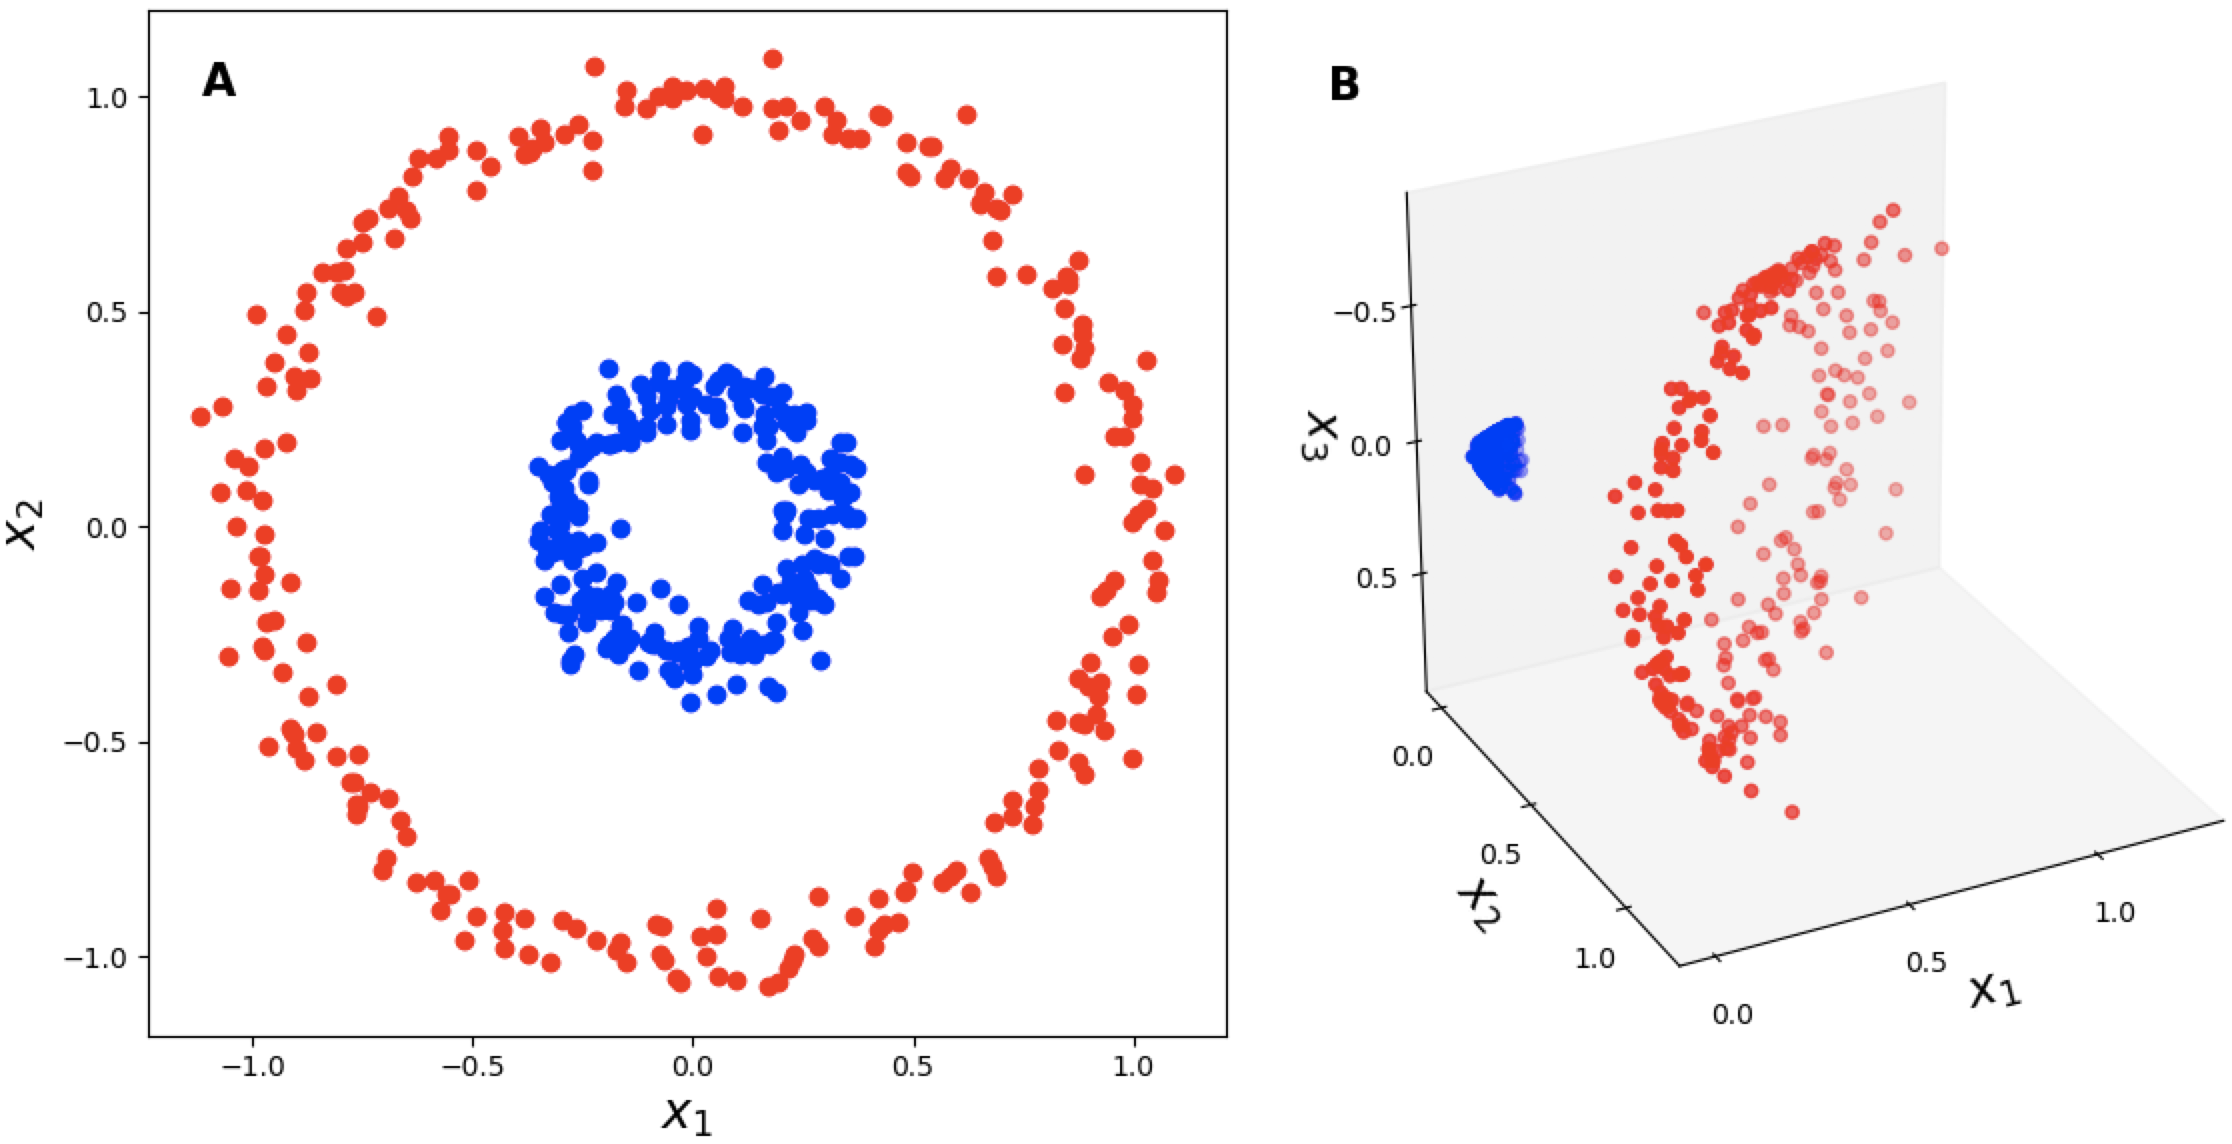
\includegraphics[height=4cm]{figures/kernel_trick2}
    \caption{Transformation $\Psi : \bx \to \Psi(\bx)$ (illustration in presence of existing labels)}
  \end{figure}

\end{frame}

\begin{frame}
  \frametitle{Kernel-PCA}

  \begin{block}{Kernel PCA Model}
    Assume a non linear transformation $ \Psi(\mathbf{x}_i) \text{ where } \Psi : \mathbb{R}^p \to \mathbb{R}^n$,  then perform linear PCA, with $\bU$ a \alert{\bf $n\times q$} orthonormal matrix
    \[
      \Phi(\bx) = \bU^\top \Psi(\bx-\bmu) = \tilde\bx
    \]
  \end{block}

  \begin{block}{Kernel trick}
    Never calculate  $\Psi(\bx_i)$ thanks to the kernel trick:
    \[K = k(\mathbf{x},\mathbf{y}) = (\Psi(\mathbf{x}),\Psi(\mathbf{y})) = \Psi(\mathbf{x})^T\Psi(\mathbf{y}) \]
  \end{block}

  \begin{block}{Solution}
    Eigen-decomposition of the doubly centered kernel matrix $\mathbf{K} = k(\bx_i, \bx_{i'})$ 
    \[\tilde{\mathbf{K}} = 
    (\bI - \mathbf{1}\mathbf{1}^\top/n) \mathbf{K} (\bI - \mathbf{1}\mathbf{1}^\top/n) = \bU {\boldsymbol\Lambda} \bU^\top \]
  \end{block}

\end{frame}

\begin{frame}[fragile]
  \frametitle{Choice of a kernel} 

  A symmetric positive definite function $k(\mathbf{x},\mathbf{y}) \in \Rset$, which depends on the kind of \alert{\bf similarity} assumed

\begin{block}{Some common kernels}

\begin{itemize}
\item \alert{\bf Polynormial Kernel }

\[ k(\bx_i,\bx_{i'}) = (\bx_{i}^\top \bx_{i'} + c)^d \]

\item  \alert{\bf Gaussian (radial) kernel}

\[k(\bx_i,\bx_{i'}) = \exp{\frac {-\left\|\bx_i - \bx_{i'} \right\|^2}{2\sigma^2}}\]

\item  \alert{\bf Laplacian kernel}

\[k(\bx_i,\bx_{i'}) = \exp{\frac {-\left\|\bx_i - \bx_{i'} \right\|}{\sigma}}\]

\end{itemize}
\end{block}

\rsa Kernel PCA suffers from the choice of the Kernel to correctly

\end{frame}


\begin{frame}[fragile]
  \frametitle{Example on scRNA} 
  \framesubtitle{Run the fit}

\begin{knitrout}\scriptsize
\definecolor{shadecolor}{rgb}{0.969, 0.969, 0.969}\color{fgcolor}\begin{kframe}
\begin{alltt}
\hlstd{scRNA_expr} \hlkwb{<-} \hlstd{scRNA} \hlopt \hlstd{dplyr}\hlopt{::}\hlkwd{select}\hlstd{(}\hlopt{-}\hlstd{cell_type)} \hlopt \hlkwd{as.matrix}\hlstd{()}

\hlstd{kPCA_radial} \hlkwb{<-}
  \hlkwd{kpca}\hlstd{(scRNA_expr,} \hlkwc{kernel} \hlstd{=} \hlstr{"rbfdot"}\hlstd{,} \hlkwc{features} \hlstd{=} \hlnum{2}\hlstd{,} \hlkwc{kpar} \hlstd{=} \hlkwd{list}\hlstd{(}\hlkwc{sigma} \hlstd{=} \hlnum{0.5}\hlstd{))} \hlopt
  \hlkwd{pcv}\hlstd{()} \hlopt \hlkwd{as.data.frame}\hlstd{()} \hlopt
  \hlkwd{add_column}\hlstd{(}\hlkwc{kernel} \hlstd{=} \hlstr{"Radial"}\hlstd{)} \hlopt
  \hlkwd{add_column}\hlstd{(}\hlkwc{cell_type} \hlstd{= scRNA}\hlopt{$}\hlstd{cell_type)}

\hlstd{kPCA_linear} \hlkwb{<-}
  \hlkwd{kpca}\hlstd{(scRNA_expr,} \hlkwc{kernel} \hlstd{=} \hlstr{"vanilladot"}\hlstd{,} \hlkwc{features} \hlstd{=} \hlnum{2}\hlstd{,} \hlkwc{kpar} \hlstd{=} \hlkwd{list}\hlstd{())} \hlopt
  \hlkwd{pcv}\hlstd{()} \hlopt \hlkwd{as.data.frame}\hlstd{()} \hlopt
  \hlkwd{add_column}\hlstd{(}\hlkwc{kernel} \hlstd{=} \hlstr{"Linear"}\hlstd{)} \hlopt
  \hlkwd{add_column}\hlstd{(}\hlkwc{cell_type} \hlstd{= scRNA}\hlopt{$}\hlstd{cell_type)}

\hlstd{kPCA_polydot} \hlkwb{<-} \hlkwd{kpca}\hlstd{(scRNA_expr,} \hlkwc{kernel} \hlstd{=} \hlstr{"polydot"}\hlstd{,} \hlkwc{features} \hlstd{=} \hlnum{2}\hlstd{,} \hlkwc{kpar} \hlstd{=} \hlkwd{list}\hlstd{(}\hlkwc{degree} \hlstd{=} \hlnum{3}\hlstd{))} \hlopt
  \hlkwd{pcv}\hlstd{()} \hlopt \hlkwd{as.data.frame}\hlstd{()} \hlopt
  \hlkwd{add_column}\hlstd{(}\hlkwc{kernel} \hlstd{=} \hlstr{"Polynomial"}\hlstd{)} \hlopt
  \hlkwd{add_column}\hlstd{(}\hlkwc{cell_type} \hlstd{= scRNA}\hlopt{$}\hlstd{cell_type)}

\hlstd{kPCA_laplacedot} \hlkwb{<-} \hlkwd{kpca}\hlstd{(scRNA_expr,} \hlkwc{kernel} \hlstd{=} \hlstr{"laplacedot"}\hlstd{,} \hlkwc{features} \hlstd{=} \hlnum{2}\hlstd{)} \hlopt
  \hlkwd{pcv}\hlstd{()} \hlopt \hlkwd{as.data.frame}\hlstd{()} \hlopt
  \hlkwd{add_column}\hlstd{(}\hlkwc{kernel} \hlstd{=} \hlstr{"Laplace"}\hlstd{)} \hlopt
  \hlkwd{add_column}\hlstd{(}\hlkwc{cell_type} \hlstd{= scRNA}\hlopt{$}\hlstd{cell_type)}
\end{alltt}
\end{kframe}
\end{knitrout}
\end{frame}

\begin{frame}[fragile]
  \frametitle{Example on scRNA} 
  \framesubtitle{Compare the projections}

\begin{knitrout}\scriptsize
\definecolor{shadecolor}{rgb}{0.969, 0.969, 0.969}\color{fgcolor}\begin{kframe}
\begin{alltt}
\hlkwd{rbind}\hlstd{(kPCA_linear, kPCA_polydot, kPCA_radial, kPCA_laplacedot)} \hlopt
  \hlkwd{ggplot}\hlstd{(}\hlkwd{aes}\hlstd{(}\hlkwc{x} \hlstd{= V1,} \hlkwc{y} \hlstd{= V2,} \hlkwc{color} \hlstd{= cell_type))} \hlopt{+}
  \hlkwd{geom_point}\hlstd{(}\hlkwc{size}\hlstd{=}\hlnum{1.25}\hlstd{)} \hlopt{+} \hlkwd{guides}\hlstd{(}\hlkwc{colour} \hlstd{=} \hlkwd{guide_legend}\hlstd{(}\hlkwc{override.aes} \hlstd{=} \hlkwd{list}\hlstd{(}\hlkwc{size}\hlstd{=}\hlnum{6}\hlstd{)))} \hlopt{+}
  \hlkwd{facet_wrap}\hlstd{(.}\hlopt{~}\hlstd{kernel,} \hlkwc{scales} \hlstd{=} \hlstr{'free'}\hlstd{)} \hlopt{+} \hlkwd{labs}\hlstd{(}\hlkwc{x} \hlstd{=} \hlstr{''}\hlstd{,} \hlkwc{y} \hlstd{=} \hlstr{''}\hlstd{)}
\end{alltt}
\end{kframe}
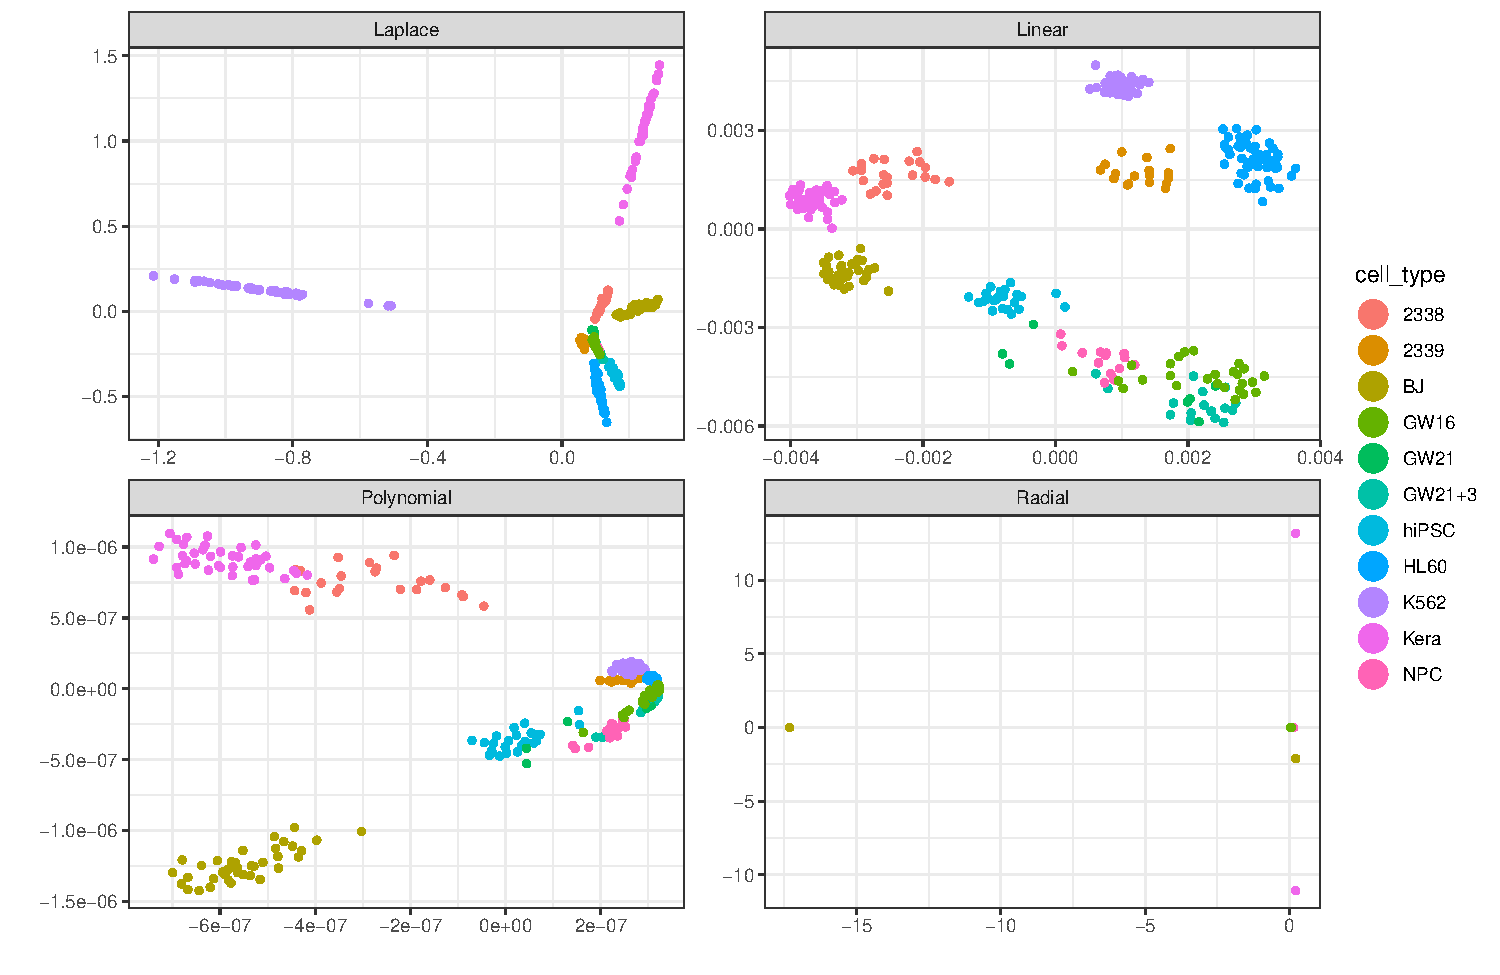
\includegraphics[width=.8\textwidth]{figures/kPCA_scRNA_kernel_plot-1} 

\end{knitrout}

\end{frame}


\subsection{Non-negative matrix factorization}



\begin{frame}
  \frametitle{Non-negative Matrix Factorization -- NMF}
  
  \begin{block}{Setup}
  Assume that $\bX$ contains only non-negative entries (i.e. $\geq 0$).
  \end{block}
  
  \begin{block}{Model}
   \alert{\bf Linear assumption + non-negativity constraints on both $\bV$ and $\tilde\bx$}
    \begin{align*}
      \Phi(\bx) & = \bV^\top(\bx-\bmu)  = \tilde\bx \\  
      \bx \simeq \tilde{\Phi}(\tilde\bx) & = \bmu + \bV \tilde\bx
    \end{align*}

  For the whole data matrix $\bX$,
  \[
    \hat{\bX} = \mathbf{1}_n \bmu^\top   + \underbrace{\tilde\bX}_{\mathbf{F}, \text{ the factors}} \bV^\top 
  \]
  \end{block}

\end{frame}

\begin{frame}[fragile]
  \frametitle{NMF reconstruction errors}
  
  Build $\hat{\mathbf{X}} = \mathbf{FV}^\top$ to minimize a distance $D(\hat{\mathbf{X}}, \mathbf{X})$! \alert{Several choice, e.g:}
    \begin{itemize}
    \item Least-square loss (distance measured by Frobenius norm)
    \[ \hat{\mathbf{X}}^{\text{ls}} =  \argmin_{\substack{\mathbf{F}\in\mathcal{M}(\Rset_+)_{n,q}\\\mathbf{V}\in\mathcal{M}(\Rset_+)_{p,q}}} \left\|     \mathbf{X} - \mathbf{FV}^\top \right\|_F^2,
\]
    \item Kullback-Leibler divergence ("distance" between distribution)
    \begin{align*}
    \hat{\mathbf{X}}^{\text{kl}} & =  \argmin_{\substack{\mathbf{F}\in\mathcal{M}(\Rset_+)_{n,q}\\ \mathbf{V}\in\mathcal{M}(\Rset_+)_{p,q}}} \sum_{i,j} x_{ij} \log(\frac{x_{ij}}{(\mathbf{F}\bV^\top)_{ij}}) + (\mathbf{F}\bV^\top)_{ij} \\
    & = \argmax_{\substack{\mathbf{F}\in\mathcal{M}(\Rset_+)_{n,q}\\ \mathbf{V}\in\mathcal{M}(\Rset_+)_{p,q}}} \sum_{i,j} x_{ij} \log((\mathbf{F}\bV^\top)_{ij}) - (\mathbf{F}\bV^\top)_{ij},\\
    \end{align*}
    \rsa log-likelihood of a Poisson distribution with mean $(\mathbf{F}\bV^\top)_{ij}$.
    \end{itemize}
\end{frame}

\begin{frame}[fragile,allowframebreaks]
  \frametitle{Example on 'mollusk'} 

\paragraph{Run the fit}

\begin{knitrout}\scriptsize
\definecolor{shadecolor}{rgb}{0.969, 0.969, 0.969}\color{fgcolor}\begin{kframe}
\begin{alltt}
\hlstd{nmf_KL} \hlkwb{<-} \hlstd{mollusk} \hlopt \hlstd{dplyr}\hlopt{::}\hlkwd{select}\hlstd{(}\hlopt{-}\hlstd{site,} \hlopt{-}\hlstd{season)} \hlopt
  \hlkwd{nmf}\hlstd{(}\hlkwc{rank} \hlstd{=} \hlnum{2}\hlstd{,} \hlkwc{method} \hlstd{=} \hlstr{'brunet'}\hlstd{)} \hlopt \hlkwd{basis}\hlstd{()} \hlopt
  \hlkwd{as.data.frame}\hlstd{()} \hlopt \hlkwd{add_column}\hlstd{(}\hlkwc{algo} \hlstd{=} \hlstr{"KL"}\hlstd{)} \hlopt \hlkwd{add_column}\hlstd{(}\hlkwc{site} \hlstd{= mollusk}\hlopt{$}\hlstd{site)}
\hlstd{nmf_LS} \hlkwb{<-} \hlstd{mollusk} \hlopt \hlstd{dplyr}\hlopt{::}\hlkwd{select}\hlstd{(}\hlopt{-}\hlstd{site,} \hlopt{-}\hlstd{season)} \hlopt
  \hlkwd{nmf}\hlstd{(}\hlkwc{rank} \hlstd{=} \hlnum{2}\hlstd{,} \hlkwc{method} \hlstd{=} \hlstr{'lee'}\hlstd{)} \hlopt \hlkwd{basis}\hlstd{()} \hlopt
  \hlkwd{as.data.frame}\hlstd{()} \hlopt \hlkwd{add_column}\hlstd{(}\hlkwc{algo} \hlstd{=} \hlstr{"LS"}\hlstd{)} \hlopt \hlkwd{add_column}\hlstd{(}\hlkwc{site} \hlstd{= mollusk}\hlopt{$}\hlstd{site)}
\end{alltt}
\end{kframe}
\end{knitrout}

\paragraph{Compare algorithms}

\begin{knitrout}\scriptsize
\definecolor{shadecolor}{rgb}{0.969, 0.969, 0.969}\color{fgcolor}\begin{kframe}
\begin{alltt}
\hlkwd{rbind}\hlstd{(nmf_KL, nmf_LS)} \hlopt
  \hlkwd{ggplot}\hlstd{(}\hlkwd{aes}\hlstd{(}\hlkwc{x} \hlstd{= V1,} \hlkwc{y} \hlstd{= V2,} \hlkwc{color} \hlstd{= site))} \hlopt{+}
     \hlkwd{geom_point}\hlstd{(}\hlkwc{size}\hlstd{=}\hlnum{1.25}\hlstd{)} \hlopt{+}
     \hlkwd{guides}\hlstd{(}\hlkwc{colour} \hlstd{=} \hlkwd{guide_legend}\hlstd{(}\hlkwc{override.aes} \hlstd{=} \hlkwd{list}\hlstd{(}\hlkwc{size}\hlstd{=}\hlnum{6}\hlstd{)))} \hlopt{+}
  \hlkwd{facet_wrap}\hlstd{(.}\hlopt{~}\hlstd{algo,} \hlkwc{scales} \hlstd{=} \hlstr{'free'}\hlstd{)}
\end{alltt}
\end{kframe}
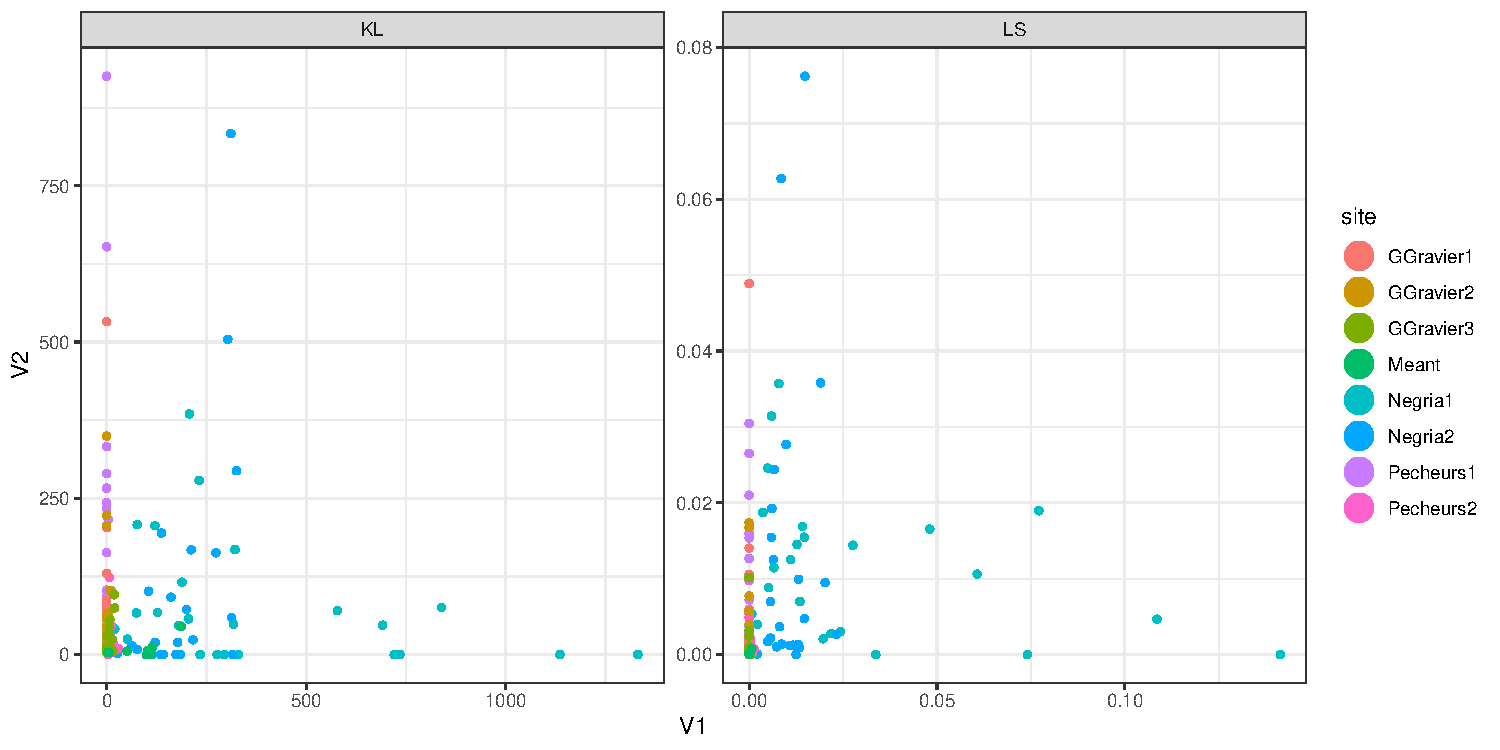
\includegraphics[width=\textwidth]{figures/NMF_mollusk_algo_plot-1} 

\end{knitrout}

\end{frame}


\begin{frame}
  \frametitle{NMF: limitations}

  \begin{block}{Caveats}  
    \begin{itemize}
      \item Basis $\bV$ formed by standard NMF is not orthogonal!
      \item Visualization is questionable \dots
      \item Used to performed matrix factorization rather than exploratory analysis
    \end{itemize}
  \end{block}

  \bigskip

  \begin{block}{Other model-based approaches}
    Use a probabilistic-based model to better described non-negative data
    \begin{itemize}
      \item[\rsa] add Zero-inflation, surdispersion (Poisson-lognormal model, Poisson-Gamma, etc)
    \end{itemize}
  \end{block}
  
\end{frame}



\subsection{Other directions}

\begin{frame}
  \frametitle{Other approaches}
  \framesubtitle{Linear model with other constraints}
    
    Let $\bV$ be a $p\times q$ matrix and $\tilde \bx \in \Rset^q$
    \begin{equation*}
      \bx \simeq  \bmu + \sum_{j=1}^q \tilde x^j \bV^j = \bmu + \bV \tilde\bx
    \end{equation*}
  
    Apply other constraints on $\bV$ and or the factor/representation $\tilde\bx$
    \begin{itemize}
      \item $\bV$ sparse, possibly orthogonal: \alert{\bf sparse PCA}\\
\begin{knitrout}\scriptsize
\definecolor{shadecolor}{rgb}{0.969, 0.969, 0.969}\color{fgcolor}\begin{kframe}
\begin{alltt}
\hlkwd{library}\hlstd{(sparsepca)}
\end{alltt}
\end{kframe}
\end{knitrout}
      \item $\tilde \bx$ sparse : \alert{\bf Dictionary learning}
\begin{knitrout}\scriptsize
\definecolor{shadecolor}{rgb}{0.969, 0.969, 0.969}\color{fgcolor}\begin{kframe}
\begin{alltt}
\hlkwd{library}\hlstd{(SPAMS)}
\end{alltt}
\end{kframe}
\end{knitrout}
      \item ($\tilde X^j, \tilde X^\ell$) independent : \alert{\bf Independent Component Anaysis}
\begin{knitrout}\scriptsize
\definecolor{shadecolor}{rgb}{0.969, 0.969, 0.969}\color{fgcolor}\begin{kframe}
\begin{alltt}
\hlkwd{library}\hlstd{(fastICA)}
\end{alltt}
\end{kframe}
\end{knitrout}
    \end{itemize}

\end{frame}
 
\begin{frame}
   \frametitle{Auto-encoders}
   
   \begin{block}{Highly non-linear model}

      Find $\Phi$ and $\tilde\Phi$ with \alert{\bf two} neural-networks, controlling the error.

      \begin{equation*}
        \epsilon(\bX, \hat \bX ) = \sum_{i=1}^n \left\| \bx_i - \tilde{\Phi}(\Phi(\bx_i)) \right\|^2 \alert{\bf + \text{regularization}(\Phi, \tilde\Phi)}
      \end{equation*}

      \begin{itemize}
         \item \# layers and neurons determine the \alert{\bf model complexity}
         \item Need regularization to avoid \alert{\bf overfitting}
         \item  Fitted with optimization tools like stochastic gradient descent
         \item Require much \alert{more data} and more computational \alert{resources}
         \item \alert{\bf Interpretation questionable}
      \end{itemize}

   \end{block}

Some Python equivalents of (torch, pytorch, tensorflow):
 
\begin{knitrout}\scriptsize
\definecolor{shadecolor}{rgb}{0.969, 0.969, 0.969}\color{fgcolor}\begin{kframe}
\begin{alltt}
\hlkwd{library}\hlstd{(keras)}

\hlkwd{library}\hlstd{(torch)}
\end{alltt}
\end{kframe}
\end{knitrout}

\rsa First rudimentary steps with auto-encoders during next homework

\end{frame}


%% ==========================================================================
\section{Motivated by relation preservation}
%% ==========================================================================


\begin{frame}
    \frametitle{Pairwise Relation}

    Focus on pairwise relation $\mathcal{R}(\bx_i, \bx_{i'})$.

    \begin{block}{Distance Preservation}
      \begin{itemize}
    \item  Construct a map $\Phi$ from the space $\Rset^{p}$ into a space $\Rset^{q}$ of \alert{smaller dimension}:
      \begin{align*}
      \Phi:\quad & \Rset^p \to \Rset^{q}, q \ll p\\
               & \bx \mapsto \Phi(\bx)
      \end{align*}
      \begin{equation*}
      \text{such that} \quad \mathcal{R}(\bx_i, \bx_{i'}) \sim\mathcal{R'}(\tilde\bx_i, \tilde\bx_{i'})
      \end{equation*}
    \end{itemize}
  \end{block}

  \begin{block}{Multidimensional scaling}
    Try to preserve inner product related to the distance (e.g. Euclidean)
  \end{block}

  \vfill

  \begin{block}{t-SNE -- Stochastic Neighborhood Embedding}
    Try to preserve relations with close neighbors with Gaussian kernel
  \end{block}

\end{frame}


\subsection{Multidimensional Scaling}



\begin{frame}{Multidimensional scaling}
  \framesubtitle{a.k.a Principale Coordinates Analysis}

  \begin{block}{Problem setup}
  Consider a collection of points $\bx_i\in\Rset^p$ and assume either 
  \begin{itemize}
  \item $D = d_{ii'}$ a $n\times n$ dissimilarity matrix, or
  \item $S = s_{ii'}$ a $n\times n$ similarity matrix, or
  \end{itemize}
  \rsa \alert{\bf Goal:} find $\tilde\bx_i\in\Rset^q$ while preserving S/D in the latent space\\
  
  \rsa we don't need access to the original position in $\Rset^p$ (only $D$ or $S$).
  \end{block}
  
  \begin{block}{Classical MDS model}
    Measure similarities with the (centered) \alert{\bf inner product} and minimize 
    \begin{equation*}
      \sum_{i\neq i'} \left( (\bx_i - \bmu)^\top (\bx_i - \bmu) - \tilde\bx_i^\top \tilde\bx_{i'} \right)^2,
    \end{equation*}
    while assuming a linear model $\tilde\bx = \Phi(\bx) = \bV^\top (\bx_i - \bmu)$, with $\bV$ a $p \times q$ orthonormal matrix.
  \end{block}

\end{frame}

\begin{frame}
  \frametitle{Classical MDS: solution}

  With the linear model $\tilde\bx = \Phi(\bx) = \bV^\top (\bx_i - \bmu)$, we waim at minimizing
  \begin{align*}
    \textrm{Stress}(\tilde\bx_i) = & \sum_{i\neq i'}  \left( (\bx_i - \bmu)^\top (\bx_{i'} - \bmu) - \tilde\bx_i^\top \tilde\bx_{i'} \right)^2, \\
    = & \sum_{i\neq i'} \left( (\bx_i - \bmu)^\top (\bx_{i'} - \bmu) -  (\bx_i - \bmu)^\top \bV \bV^\top (\bx_{i'} - \bmu) \right)^2,
    \end{align*}

  It can be showed that  $\displaystyle \minimize_{\bmu\in\Rset^p, \bV\in\mathcal{O}_{pq}} \textrm{Stress}(\tilde\bx_i)$ is dual to principal component analysis and leads to
  \[
    \tilde\bX = \bX^c \bV = \bU\bD\bV^\top \bV = \bU\bD.
  \]
  
  \alert{\rsa The principal coordinates in $\Rset^q$ correspond to the scores of $n$ individual projected on the first $q$ principal components.}
\end{frame}


\begin{frame}
  \frametitle{Metric Dimension Scalings}
  
  \paragraph{Idea to generalize classical MDS:} preserving similarities in term of \alert{\bf inner product} amounts to preserve dissimilarity in terms of Euclidean distance

  \begin{block}{Least-square/Kruskal-Shephard scaling}<2->
      Use a distance base formulation with the following loss (Stress) function:
      \begin{equation*}
        \text{Stress}^{SK} = \sum_{i\neq i'} \left(d_{ii'} - \|\tilde\bx_i - \tilde\bx_{i'}\| \right)^2,
      \end{equation*}
      \begin{itemize}
        \item[\rsa] Almost equivalent to classical MDS when $d$ is the Euclidean distance
        \item[\rsa] Generalize to any \alert{\bf quantitative} dissimilarity/distance $d$
      \end{itemize}
  \end{block}

  \begin{block}{Sammong mapping - \textcolor{black}{Variant of the loss (Stress) function}}<3>
    \vspace{-.5cm}
      \begin{equation*}
        \text{Stress}^{SM} = \sum_{i\neq i'} \frac{\left(d_{ii'} - \|\tilde\bx_i - \tilde\bx_{i'}\| \right)^2}{d_{ii'}}.
      \end{equation*}
  \end{block}

\end{frame}


\begin{frame}
  \frametitle{Non-Metric Dimension Scalings}
  
  \paragraph{Idea:} dissimilarities are often only knows by their rank order

  \begin{block}{Shephard-Kruskal non-metric scaling}
      \begin{equation*}
        \text{Stress}^{NM} = \sum_{i\neq i'} \frac{\left(d_{ii'} - f(d_{ii'}) \right)^2}{\sum_{i\neq i'} d_{ii'}^2},
      \end{equation*}
      where $f$ is an arbitrary increasing function preserving the order
      \begin{itemize}
        \item[\rsa] Only the order it required
        \item[\rsa] $f$ act a isotonic regression curve for the $d_{ii'}$. 
      \end{itemize}
  \end{block}

\end{frame}


\begin{frame}[fragile,allowframebreaks]
  \frametitle{Example on 'mollusk'} 

\paragraph{Run the fit}

\begin{knitrout}\scriptsize
\definecolor{shadecolor}{rgb}{0.969, 0.969, 0.969}\color{fgcolor}\begin{kframe}
\begin{alltt}
\hlstd{mollusk_ab} \hlkwb{<-} \hlstd{mollusk} \hlopt \hlstd{dplyr}\hlopt{::}\hlkwd{select}\hlstd{(}\hlopt{-}\hlstd{site,} \hlopt{-}\hlstd{season)} \hlopt  \hlkwd{as.matrix}\hlstd{()}

\hlstd{mmds_euclidean} \hlkwb{<-} \hlkwd{cmdscale}\hlstd{(}\hlkwd{dist}\hlstd{(mollusk_ab))} \hlopt
  \hlkwd{as.data.frame}\hlstd{()} \hlopt \hlkwd{add_column}\hlstd{(}\hlkwc{type} \hlstd{=} \hlstr{"mMDS, Euclidean"}\hlstd{)} \hlopt \hlkwd{add_column}\hlstd{(}\hlkwc{site} \hlstd{= mollusk}\hlopt{$}\hlstd{site)}

\hlstd{mmds_canberra} \hlkwb{<-} \hlkwd{cmdscale}\hlstd{(}\hlkwd{dist}\hlstd{(mollusk_ab,} \hlkwc{method} \hlstd{=} \hlstr{"canberra"}\hlstd{))} \hlopt
  \hlkwd{as.data.frame}\hlstd{()} \hlopt \hlkwd{add_column}\hlstd{(}\hlkwc{type} \hlstd{=} \hlstr{"mMDS, Canberra"}\hlstd{)} \hlopt \hlkwd{add_column}\hlstd{(}\hlkwc{site} \hlstd{= mollusk}\hlopt{$}\hlstd{site)}

\hlstd{nmds} \hlkwb{<-} \hlstd{MASS}\hlopt{::}\hlkwd{isoMDS}\hlstd{(}\hlkwd{dist}\hlstd{(mollusk_ab,} \hlstr{"canberra"}\hlstd{))}\hlopt{$}\hlstd{points} \hlopt
  \hlkwd{as.data.frame}\hlstd{()} \hlopt \hlkwd{add_column}\hlstd{(}\hlkwc{type} \hlstd{=} \hlstr{"nmMDS"}\hlstd{)} \hlopt \hlkwd{add_column}\hlstd{(}\hlkwc{site} \hlstd{= mollusk}\hlopt{$}\hlstd{site)}
\end{alltt}
\begin{verbatim}
## initial  value 39.689470 
## iter   5 value 32.736128
## final  value 32.587709 
## converged
\end{verbatim}
\end{kframe}
\end{knitrout}

\paragraph{Compare type of MDS}

\begin{knitrout}\scriptsize
\definecolor{shadecolor}{rgb}{0.969, 0.969, 0.969}\color{fgcolor}\begin{kframe}
\begin{alltt}
\hlkwd{rbind}\hlstd{(mmds_euclidean, mmds_canberra, nmds)} \hlopt
  \hlkwd{ggplot}\hlstd{(}\hlkwd{aes}\hlstd{(}\hlkwc{x} \hlstd{= V1,} \hlkwc{y} \hlstd{= V2,} \hlkwc{color} \hlstd{= site))} \hlopt{+}
     \hlkwd{geom_point}\hlstd{(}\hlkwc{size}\hlstd{=}\hlnum{1.25}\hlstd{)} \hlopt{+}
     \hlkwd{guides}\hlstd{(}\hlkwc{colour} \hlstd{=} \hlkwd{guide_legend}\hlstd{(}\hlkwc{override.aes} \hlstd{=} \hlkwd{list}\hlstd{(}\hlkwc{size}\hlstd{=}\hlnum{6}\hlstd{)))} \hlopt{+}
  \hlkwd{facet_wrap}\hlstd{(.}\hlopt{~}\hlstd{type,} \hlkwc{scales} \hlstd{=} \hlstr{'free'}\hlstd{)}
\end{alltt}
\end{kframe}
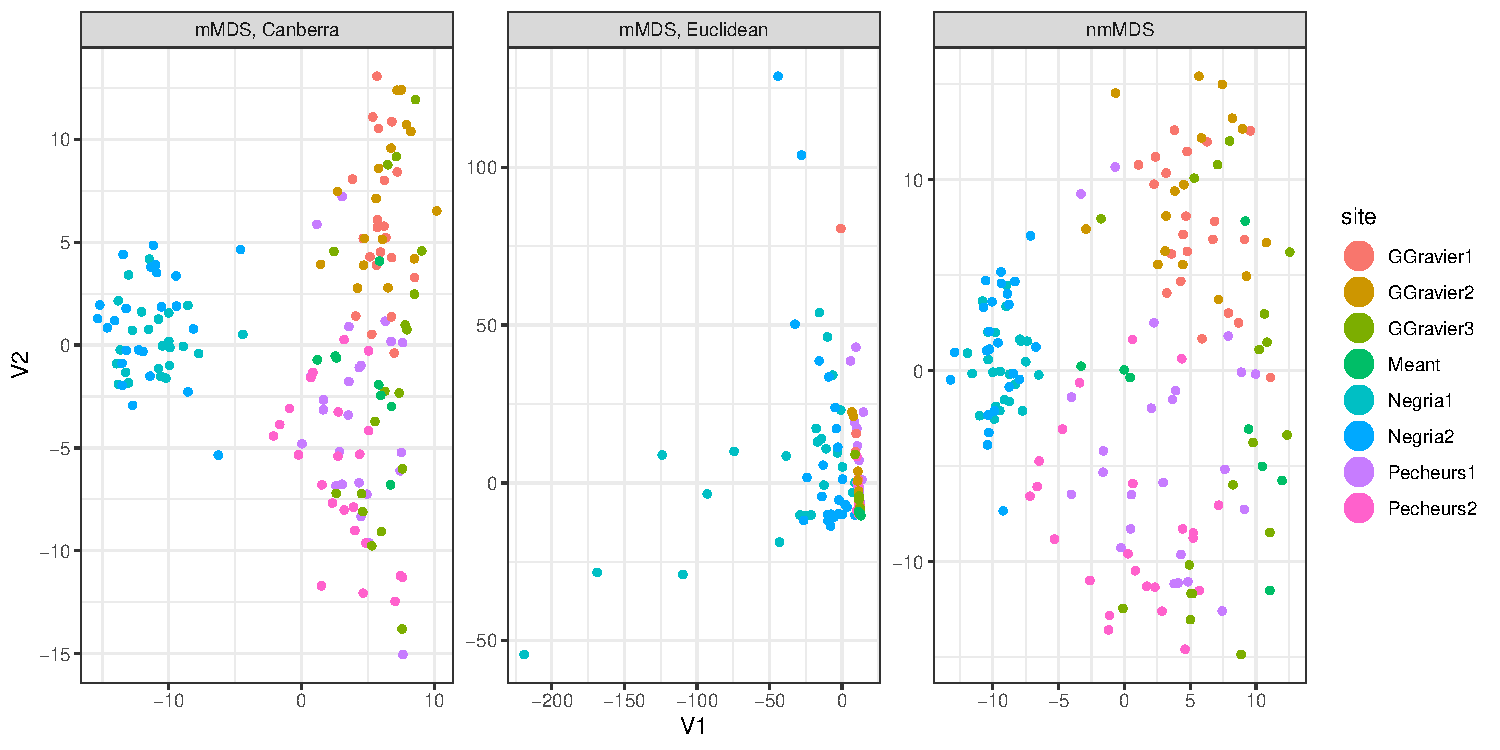
\includegraphics[width=.9\textwidth]{figures/MDS_mollusk_plot-1} 

\end{knitrout}

\end{frame}

\subsection{Stochastic Neighborhood Embedding}



\begin{frame}{Stochastic Neighbor Embedding}

Let $(\bx_1, \hdots, \bx_n)$ be the original points in $\mathbb{R}^p$, and consider a similarities:

\[p_{i{i'}} =  (p_{i | {i'}} + p_{{i'} | i})/ 2n\]
where
\begin{align*}
  p_{i | {i'}} & = \frac{ \exp(- \| \bx_i - \bx_{i'} \|^2 / 2 \sigma_i^2 ) }{\sum_{k \neq i} \exp(- \| \bx_k - \bx_{i'} \|^2 / 2 \sigma_k^2)}, \\
  & = \frac{ \exp(- d_{ii'}^2 / 2 \sigma_i^2 ) }{\sum_{k \neq i} \exp(- d_{ki'}^2 / 2 \sigma_k^2)}
\end{align*}

\vfill

\begin{itemize}
\item[\rsa] SNE to preserve relations with close neighbors with Gaussian kernel
\item[\rsa] $\sigma$ smooths the data (linked to the regularity of the target manifold)
\end{itemize}

\end{frame}

\begin{frame}{The perplexity parameter}

The variance $\sigma_i^2$ should adjust to local densities (neighborhood of point $i$)

\begin{block}{Perplexity: a smoothed effective number of neighbors}
The perplexity is defined by
$$
  Perp(p_i) = 2^{H(p_i)}, \qquad H(p_i) = -\sum_{j=1}^{n} p_{j|i} \log_2 p_{j|i}
$$
where $H$ is the Shannon entropy of $p_i=(p_{1|i},\hdots,p_{n|i})$.\\
\end{block}

\vfill

\rsa SNE performs a binary search for the value of $\sigma_i$ that produces a $p_i$ with a fixed perplexity that is specified by the user.

\end{frame}

\begin{frame}{tSNE and Student / Cauchy kernels}

Consider $(\tilde\bx_1,\hdots,\tilde\bx_n)$ are points in the low dimensional space $\mathbb{R}^{q=2}$

\begin{itemize}
\item Consider a similarity between points in the new representation:
$$q_{i | j} = \frac{ \exp(- \| \tilde\bx_i - \tilde\bx_j \|^2  ) }{\sum_{k \neq i} \exp(- \| \tilde\bx_k - \tilde\bx_j \|^2 )}$$
\item Robustify this kernel by using Student(1) kernels (ie Cauchy)
$$q_{i | j} = \frac{ (1 + \| \tilde\bx_i - \tilde\bx_j \|^2)^{-1}  }{\sum_{k \neq i} (1 + \| \tilde\bx_i - \tilde\bx_k \|^2)^{-1}}$$
\end{itemize}
\end{frame}

\begin{frame}{Optimizing tSNE}
\begin{itemize}
\item Minimize the KL between $p$ and $q$ so that the data representation minimizes:
$$
C(y) = \sum_{ij} KL(p_{ij},q_{ij})
$$
\item The cost function is not convex 
$$
\left[ \frac{\partial C(y)}{\partial y} \right]_i = \sum_{j} (p_{ij}-q_{ij})(y_i - y_j)
$$
\item Interpreted as the resultant force created by a set of springs between the map point $y_i$ and all other map points $\left( y_j \right)_j$. All springs exert a force along the direction $(y_i - y_j)$.
\item $(p_{ij}-q_{ij})$ is viewed as a stiffness of the force exerted by the spring between $y_i$ and $y_j$.
\end{itemize}
\end{frame}

% \begin{frame}{Customed Gradient descent}
% \begin{itemize}
% \item Gradient descent initialized by sampling map points randomly from an isotropic Gaussian with small variance centered around the origin
% \item Gradient update using
% $$
% y^{(t)} = y^{(t-1)} + \eta \frac{\partial C(y)}{\partial y} + \alpha(t) (y^{(t-1)}-y^{(t-2)})
% $$
% \item $\eta$ learning rate, $\alpha(t)$ momentum at iteration $t$.
% \item Gaussian noise is added to the map points to perform simulated annealing.
% \end{itemize}
% \end{frame}

\begin{frame}{t-SNE: pros/cons}

\begin{block}{Properties}
\begin{itemize}
\item good at preserving local distances (intra-cluster variance)
\item not so good for global representation (inter-cluster variance)
\item good at creating clusters of close points, bad at positioning clusters wrt each other
\end{itemize}
\end{block}

\begin{block}{Limitations}
\begin{itemize}
  \item importance of preprocessing: initialize with PCA and feature selection plus log transform (non linear transform)
\item percent of explained variance ? interpretation of the $q$ distribution ?
\end{itemize}
\end{block}

\end{frame}

\begin{frame}[fragile,allowframebreaks]
  \frametitle{Example on scRNA} 

\paragraph{Run the fit}

\begin{knitrout}\scriptsize
\definecolor{shadecolor}{rgb}{0.969, 0.969, 0.969}\color{fgcolor}\begin{kframe}
\begin{alltt}
\hlstd{scRNA_expr} \hlkwb{<-} \hlstd{scRNA} \hlopt \hlstd{dplyr}\hlopt{::}\hlkwd{select}\hlstd{(}\hlopt{-}\hlstd{cell_type)} \hlopt \hlkwd{as.matrix}\hlstd{()}

\hlstd{tSNE_perp2}   \hlkwb{<-} \hlkwd{Rtsne}\hlstd{(scRNA_expr,} \hlkwc{perplexity} \hlstd{=}   \hlnum{2}\hlstd{)}\hlopt{$}\hlstd{Y} \hlopt
  \hlkwd{as.data.frame}\hlstd{()} \hlopt \hlkwd{add_column}\hlstd{(}\hlkwc{perplexity} \hlstd{=} \hlnum{2}\hlstd{)} \hlopt \hlkwd{add_column}\hlstd{(}\hlkwc{cell_type} \hlstd{= scRNA}\hlopt{$}\hlstd{cell_type)}

\hlstd{tSNE_perp10}  \hlkwb{<-} \hlkwd{Rtsne}\hlstd{(scRNA_expr,} \hlkwc{perplexity} \hlstd{=}  \hlnum{10}\hlstd{)}\hlopt{$}\hlstd{Y} \hlopt
  \hlkwd{as.data.frame}\hlstd{()} \hlopt \hlkwd{add_column}\hlstd{(}\hlkwc{perplexity} \hlstd{=} \hlnum{10}\hlstd{)} \hlopt \hlkwd{add_column}\hlstd{(}\hlkwc{cell_type} \hlstd{= scRNA}\hlopt{$}\hlstd{cell_type)}

\hlstd{tSNE_perp100} \hlkwb{<-} \hlkwd{Rtsne}\hlstd{(scRNA_expr,} \hlkwc{perplexity} \hlstd{=} \hlnum{100}\hlstd{)}\hlopt{$}\hlstd{Y} \hlopt
  \hlkwd{as.data.frame}\hlstd{()} \hlopt \hlkwd{add_column}\hlstd{(}\hlkwc{perplexity} \hlstd{=} \hlnum{100}\hlstd{)} \hlopt \hlkwd{add_column}\hlstd{(}\hlkwc{cell_type} \hlstd{= scRNA}\hlopt{$}\hlstd{cell_type)}
\end{alltt}
\end{kframe}
\end{knitrout}

\paragraph{Compare perplexity}

\begin{knitrout}\scriptsize
\definecolor{shadecolor}{rgb}{0.969, 0.969, 0.969}\color{fgcolor}\begin{kframe}
\begin{alltt}
\hlkwd{rbind}\hlstd{(tSNE_perp2,tSNE_perp10,tSNE_perp100)} \hlopt
  \hlkwd{ggplot}\hlstd{(}\hlkwd{aes}\hlstd{(}\hlkwc{x} \hlstd{= V1,} \hlkwc{y} \hlstd{= V2,} \hlkwc{color} \hlstd{= cell_type))} \hlopt{+}
     \hlkwd{geom_point}\hlstd{(}\hlkwc{size}\hlstd{=}\hlnum{1.25}\hlstd{)} \hlopt{+}
     \hlkwd{guides}\hlstd{(}\hlkwc{colour} \hlstd{=} \hlkwd{guide_legend}\hlstd{(}\hlkwc{override.aes} \hlstd{=} \hlkwd{list}\hlstd{(}\hlkwc{size}\hlstd{=}\hlnum{6}\hlstd{)))} \hlopt{+}
  \hlkwd{facet_wrap}\hlstd{(.}\hlopt{~}\hlstd{perplexity,} \hlkwc{scales} \hlstd{=} \hlstr{'free'}\hlstd{)}
\end{alltt}
\end{kframe}
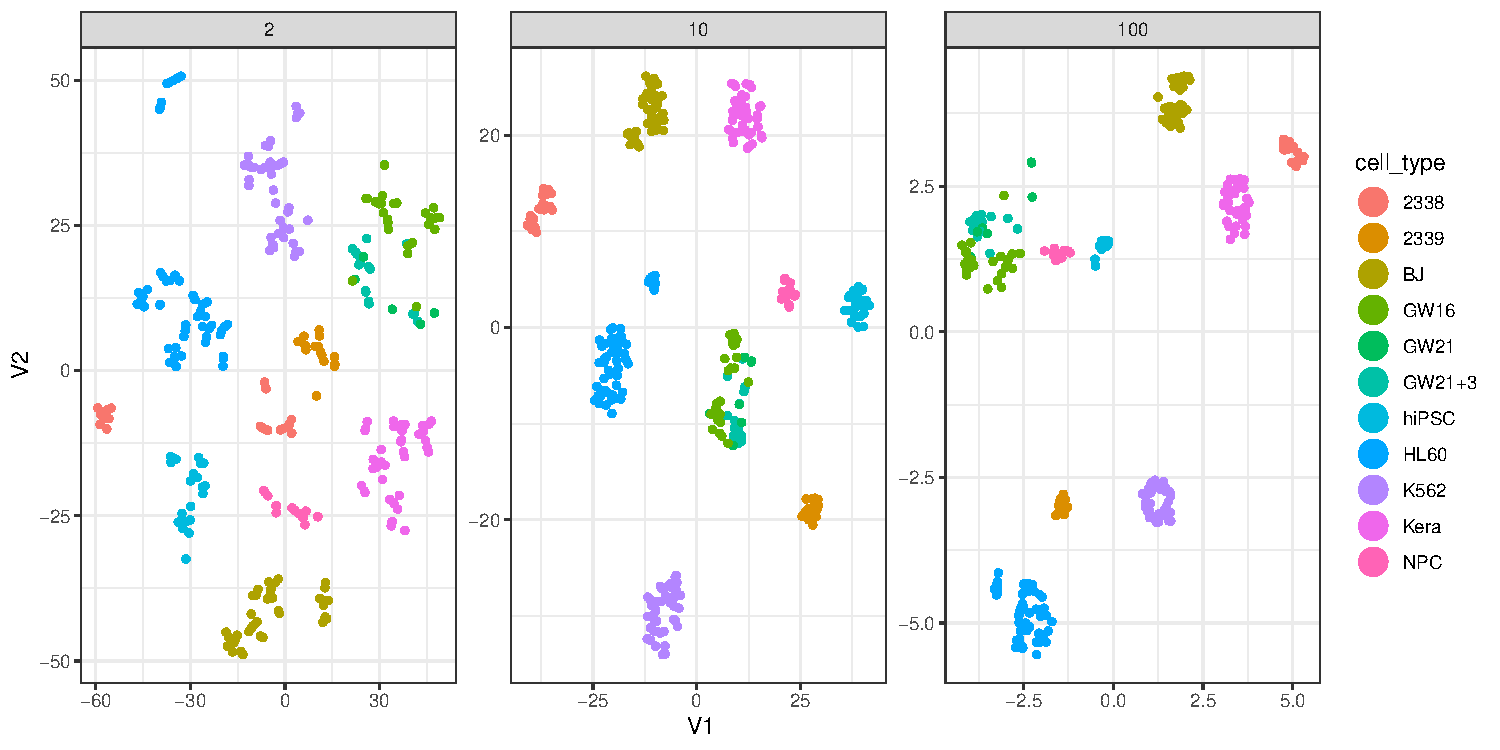
\includegraphics[width=\textwidth]{figures/tSNE_scRNA_perplexity_plot-1} 

\end{knitrout}

\end{frame}

\begin{frame}[fragile,allowframebreaks]
  \frametitle{Example on 'mollusk'} 

\paragraph{Run the fit}

\begin{knitrout}\scriptsize
\definecolor{shadecolor}{rgb}{0.969, 0.969, 0.969}\color{fgcolor}\begin{kframe}
\begin{alltt}
\hlstd{mollusk_ab} \hlkwb{<-} \hlstd{mollusk} \hlopt \hlstd{dplyr}\hlopt{::}\hlkwd{select}\hlstd{(}\hlopt{-}\hlstd{site,} \hlopt{-}\hlstd{season)} \hlopt  \hlkwd{as.matrix}\hlstd{()}

\hlstd{tSNE_perp2}   \hlkwb{<-} \hlkwd{Rtsne}\hlstd{(mollusk_ab,} \hlkwc{perplexity} \hlstd{=}   \hlnum{2}\hlstd{)}\hlopt{$}\hlstd{Y} \hlopt
  \hlkwd{as.data.frame}\hlstd{()} \hlopt \hlkwd{add_column}\hlstd{(}\hlkwc{perplexity} \hlstd{=} \hlnum{2}\hlstd{)} \hlopt \hlkwd{add_column}\hlstd{(}\hlkwc{site} \hlstd{= mollusk}\hlopt{$}\hlstd{site)}

\hlstd{tSNE_perp10}  \hlkwb{<-} \hlkwd{Rtsne}\hlstd{(}\hlkwd{log}\hlstd{(}\hlnum{1} \hlopt{+} \hlstd{mollusk_ab),} \hlkwc{perplexity} \hlstd{=}  \hlnum{10}\hlstd{)}\hlopt{$}\hlstd{Y} \hlopt
  \hlkwd{as.data.frame}\hlstd{()} \hlopt \hlkwd{add_column}\hlstd{(}\hlkwc{perplexity} \hlstd{=} \hlnum{10}\hlstd{)} \hlopt \hlkwd{add_column}\hlstd{(}\hlkwc{site} \hlstd{= mollusk}\hlopt{$}\hlstd{site)}

\hlstd{tSNE_perp50} \hlkwb{<-} \hlkwd{Rtsne}\hlstd{(}\hlkwd{log}\hlstd{(}\hlnum{1} \hlopt{+} \hlstd{mollusk_ab),} \hlkwc{perplexity} \hlstd{=} \hlnum{50}\hlstd{)}\hlopt{$}\hlstd{Y} \hlopt
  \hlkwd{as.data.frame}\hlstd{()} \hlopt \hlkwd{add_column}\hlstd{(}\hlkwc{perplexity} \hlstd{=} \hlnum{50}\hlstd{)} \hlopt \hlkwd{add_column}\hlstd{(}\hlkwc{site} \hlstd{= mollusk}\hlopt{$}\hlstd{site)}
\end{alltt}
\end{kframe}
\end{knitrout}

\paragraph{Compare perplexity}

\begin{knitrout}\scriptsize
\definecolor{shadecolor}{rgb}{0.969, 0.969, 0.969}\color{fgcolor}\begin{kframe}
\begin{alltt}
\hlkwd{rbind}\hlstd{(tSNE_perp2,tSNE_perp10,tSNE_perp50)} \hlopt
  \hlkwd{ggplot}\hlstd{(}\hlkwd{aes}\hlstd{(}\hlkwc{x} \hlstd{= V1,} \hlkwc{y} \hlstd{= V2,} \hlkwc{color} \hlstd{= site))} \hlopt{+}
     \hlkwd{geom_point}\hlstd{(}\hlkwc{size}\hlstd{=}\hlnum{1.25}\hlstd{)} \hlopt{+}
     \hlkwd{guides}\hlstd{(}\hlkwc{colour} \hlstd{=} \hlkwd{guide_legend}\hlstd{(}\hlkwc{override.aes} \hlstd{=} \hlkwd{list}\hlstd{(}\hlkwc{size}\hlstd{=}\hlnum{6}\hlstd{)))} \hlopt{+}
  \hlkwd{facet_wrap}\hlstd{(.}\hlopt{~}\hlstd{perplexity,} \hlkwc{scales} \hlstd{=} \hlstr{'free'}\hlstd{)}
\end{alltt}
\end{kframe}
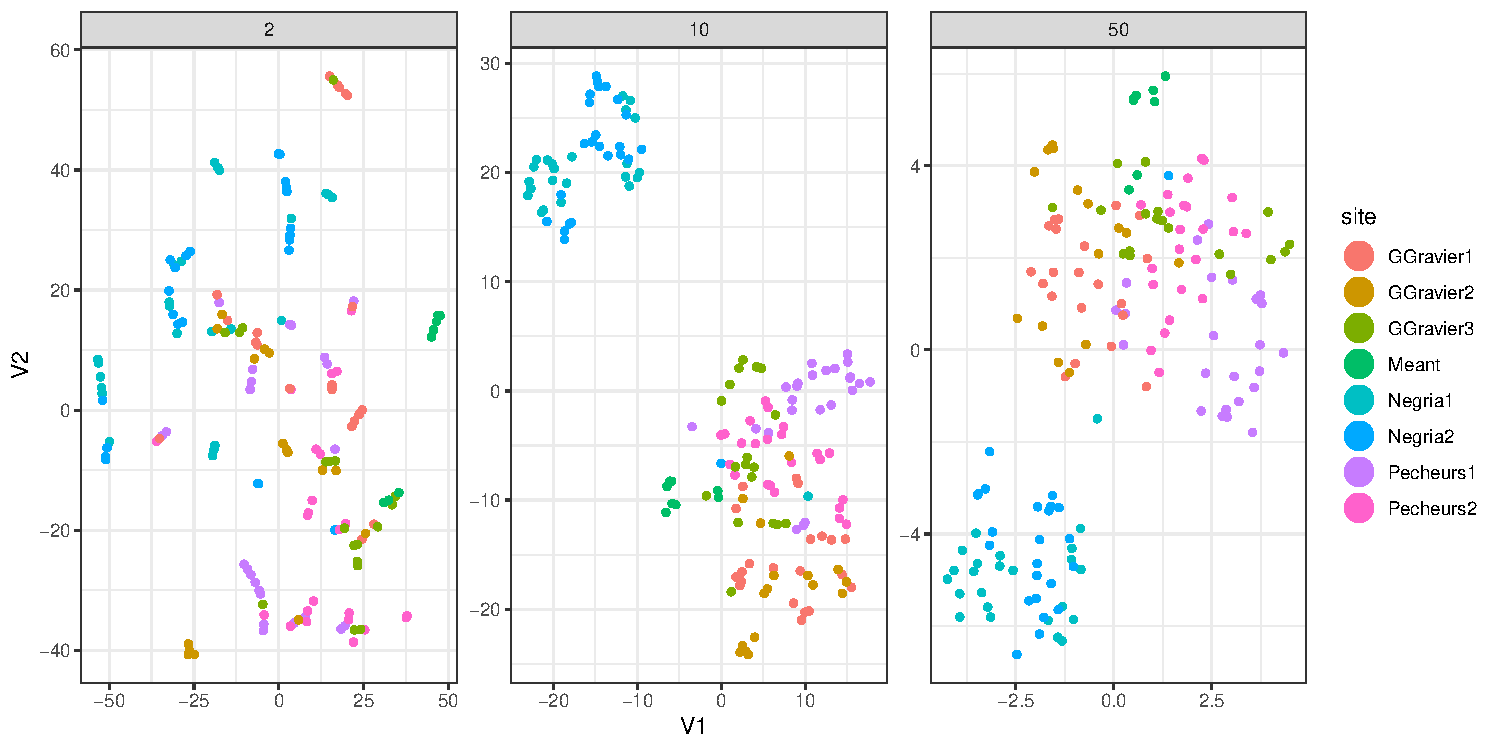
\includegraphics[width=\textwidth]{figures/tSNE_mollusk_perplexity_plot-1} 

\end{knitrout}

\end{frame}

\subsection{Other methods}



\begin{frame}
   \frametitle{Isomap}
 
   \begin{block}{Basic idea}
     \begin{itemize}
       \item MMDS performs embedding based on the pairwise Euclidean-based distance distance
       \item Isomap uses a distance induced by a neighborhood graph embedded
     \end{itemize}
   \end{block}
 
Formally, consider a neighborhood $\mathcal{N}_i$ for each point, then
\begin{equation*}
  d_{ii'} = \left\{
    \begin{array}{cc}
    + \infty & \text{ if }j \notin \mathcal{N}_i\\
    \| \bx_i - \bx_{i'} \|& \\
    \end{array}
  \right.,
\end{equation*}
 and compute the shortest path distance for each pair prior to MDS.
 
\begin{knitrout}\scriptsize
\definecolor{shadecolor}{rgb}{0.969, 0.969, 0.969}\color{fgcolor}\begin{kframe}
\begin{alltt}
\hlkwd{library}\hlstd{(vegan)}
\end{alltt}
\end{kframe}
\end{knitrout}
% 
\end{frame}

\begin{frame}[fragile,allowframebreaks]
  \frametitle{Uniform Manifold Approximation and Projection}

  \begin{itemize}
    \item Use another distance based of $k-$neighborhood graph
    \item  tends to preserve both local and glocal 
  \end{itemize}
  
\paragraph{Run the fit on scRNA}

\begin{knitrout}\scriptsize
\definecolor{shadecolor}{rgb}{0.969, 0.969, 0.969}\color{fgcolor}\begin{kframe}
\begin{alltt}
\hlstd{scRNA_expr} \hlkwb{<-} \hlstd{scRNA} \hlopt \hlstd{dplyr}\hlopt{::}\hlkwd{select}\hlstd{(}\hlopt{-}\hlstd{cell_type)} \hlopt \hlkwd{as.matrix}\hlstd{()}
\hlstd{umap_fit}   \hlkwb{<-} \hlkwd{umap}\hlstd{(scRNA_expr)}\hlopt{$}\hlstd{layout} \hlopt
  \hlkwd{as.data.frame}\hlstd{()} \hlopt \hlkwd{add_column}\hlstd{(}\hlkwc{cell_type} \hlstd{= scRNA}\hlopt{$}\hlstd{cell_type)}
\end{alltt}
\end{kframe}
\end{knitrout}

\paragraph{Visualization}

\begin{knitrout}\scriptsize
\definecolor{shadecolor}{rgb}{0.969, 0.969, 0.969}\color{fgcolor}\begin{kframe}
\begin{alltt}
\hlstd{umap_fit} \hlopt
  \hlkwd{ggplot}\hlstd{(}\hlkwd{aes}\hlstd{(}\hlkwc{x} \hlstd{= V1,} \hlkwc{y} \hlstd{= V2,} \hlkwc{color} \hlstd{= cell_type))} \hlopt{+}
     \hlkwd{geom_point}\hlstd{(}\hlkwc{size}\hlstd{=}\hlnum{1.25}\hlstd{)} \hlopt{+}
     \hlkwd{guides}\hlstd{(}\hlkwc{colour} \hlstd{=} \hlkwd{guide_legend}\hlstd{(}\hlkwc{override.aes} \hlstd{=} \hlkwd{list}\hlstd{(}\hlkwc{size}\hlstd{=}\hlnum{6}\hlstd{)))}
\end{alltt}
\end{kframe}
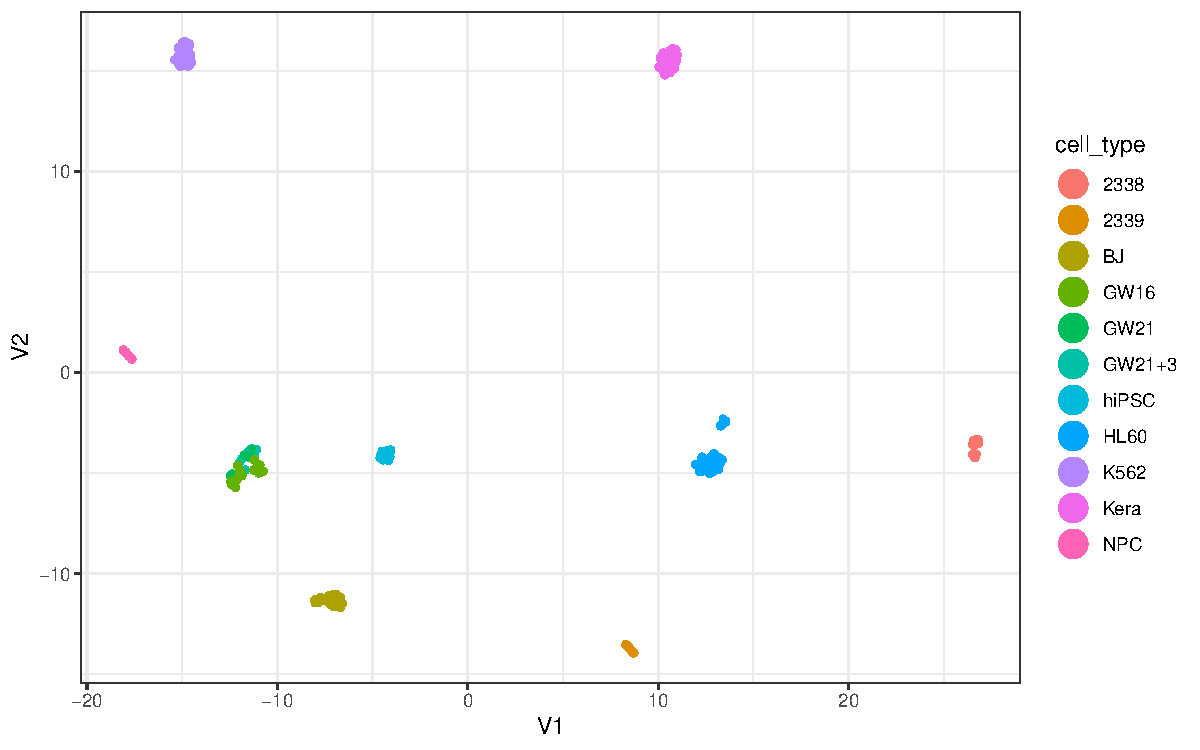
\includegraphics[width=\textwidth]{figures/plot-1} 

\end{knitrout}

\end{frame}

\begin{frame}[fragile,allowframebreaks]
  \frametitle{Example on 'mollusk'} 

\paragraph{Run the fit}

\begin{knitrout}\scriptsize
\definecolor{shadecolor}{rgb}{0.969, 0.969, 0.969}\color{fgcolor}\begin{kframe}
\begin{alltt}
\hlstd{mollusk_ab} \hlkwb{<-} \hlstd{mollusk} \hlopt \hlstd{dplyr}\hlopt{::}\hlkwd{select}\hlstd{(}\hlopt{-}\hlstd{site,} \hlopt{-}\hlstd{season)} \hlopt  \hlkwd{as.matrix}\hlstd{()}
\hlstd{umap_fit}   \hlkwb{<-} \hlkwd{umap}\hlstd{(}\hlkwd{log}\hlstd{(}\hlnum{1} \hlopt{+} \hlstd{mollusk_ab))}\hlopt{$}\hlstd{layout} \hlopt
  \hlkwd{as.data.frame}\hlstd{()} \hlopt \hlkwd{add_column}\hlstd{(}\hlkwc{site} \hlstd{= mollusk}\hlopt{$}\hlstd{site)}
\end{alltt}
\end{kframe}
\end{knitrout}

\paragraph{Visualization}

\begin{knitrout}\scriptsize
\definecolor{shadecolor}{rgb}{0.969, 0.969, 0.969}\color{fgcolor}\begin{kframe}
\begin{alltt}
\hlstd{umap_fit} \hlopt
  \hlkwd{ggplot}\hlstd{(}\hlkwd{aes}\hlstd{(}\hlkwc{x} \hlstd{= V1,} \hlkwc{y} \hlstd{= V2,} \hlkwc{color} \hlstd{= site))} \hlopt{+}
     \hlkwd{geom_point}\hlstd{(}\hlkwc{size}\hlstd{=}\hlnum{1.25}\hlstd{)} \hlopt{+}
     \hlkwd{guides}\hlstd{(}\hlkwc{colour} \hlstd{=} \hlkwd{guide_legend}\hlstd{(}\hlkwc{override.aes} \hlstd{=} \hlkwd{list}\hlstd{(}\hlkwc{size}\hlstd{=}\hlnum{6}\hlstd{)))}
\end{alltt}
\end{kframe}

\includegraphics[width=\textwidth]{figures/UMAP_mollusk_plot-1} 

\end{knitrout}

\end{frame}

%% ==========================================================================
\part{Conlusion}
%% ==========================================================================
\begin{frame}
  \frametitle{To conclude}
  
  \begin{center}
      You can play online on \href{https://projector.tensorflow.org/}{https://projector.tensorflow.org/}
  \end{center}
  
\end{frame}

% \begin{frame}[allowframebreaks]
%   \frametitle{References}
% 
%  \bibliographystyle{apalike}
% 
% \begin{small}
%   \bibliography{{../../resources/MAP573.bib}}
% \end{small}
% 
% \end{frame}

\end{document}



